\chapter{Design of a Local Path Planner} \label{cha:Design}
\vspace{-1.56em}
\section{Introduction}
The designed LPPA aims to improve the work developed in the Department of Mechanical Engineering of the KU Leuven \cite{DemeesterEtAl2012}, which has been discussed in \cref{sec:ColFreeTraj,sec:LPTreview}. A LPT is used in order to plan a motion, consisting of a fixed set of feasible trajectories starting from the robot's current pose.

The main improvement of the new LPPA is to overcome a shortcoming of the LPT from \cite{DemeesterEtAl2012}, namely the difficulty to plan feasible paths in narrow openings starting from certain poses, due to the lack of flexibility of the applied curve geometry. As only circular curves are used as a basis for the trajectories planned by this LPT, it will be referred to as the circular LPT throughout the rest of this thesis.

The solution employed to address this issue is inspired by the work of Pivtoraiko and Kelly \cite{PivtoraikoKelly2005,PivtoraikoEtAl2009,PivtoraikoKelly2012}, that has been reviewed in \cref{sec:SLreview}. Their methods describe how to generate a set of MPs in order to connect one state (robot pose) to another. The level of complexity of the trajectories depends upon the choice of the curve geometry, the basis of the MP, which will be an important design parameter.

The new LPT is created by using a Local State Lattice (LSL) (a local version of the State Lattice of Pivtoraiko and Kelly) and an obstacle-based lookup table for collision checking to obtain rapidly a set of collision-free paths. Since clothoids will ultimately be chosen as the basis of the MPs, the new LPT as developed in this thesis will be called clothoidal LPT.

The method applied can be summarized in the following steps:
\begin{enumerate}
\item Generation of a multi-size grid (fine close to the robot and coarse far from it).
\item Each grid cell in the Region Of Interest (ROI) around the origin is connected with a geometrical curve. If this path is feasible, it is added to the set of MPs.
\item To ensure a certain degree of flexibility, step 2 is repeated at certain grid cells, called Expansion Positions (EPs). By doing this, certain paths in the LSL will consist of two subsequent curves.
\item The Occupancy Grid (OG) is calculated for each path, by using the geometry of the wheelchair. A lookup table is built for this fixed set of trajectories to quickly assess if a motion is collision-free and where the collision occurs.
\item The LPPA updates each path by adjusting its length in order to be collision-free within the perceived environment.
\end{enumerate}

Steps 1 to 4 are executed offline. Step 5 is performed in real-time. The collision-free paths calculated by the LPPA are used to model the navigation intention of the wheelchair driver as explained in \cref{sec:PlanRec}. Each path receives a certain probability, reflecting its likeliness to be the true user's intention.

This chapter is structured as follows: first, the construction of the LSL is explained in \cref{sec:LSL}. Then the lookup table for collision checking with a short example of the online phase is presented in \cref{sec:LTCC}. A conceptual solution to extend the LPPA with the ability to plan a motion in a dynamic environment is presented in \cref{sec:DynPlan}. Considerations on socially compliant  path planning are provided in \cref{sec:HAPP}. Finally, a conclusion is given in \cref{sec:DesignConclusion}.

\section{Local State Lattice} \label{sec:LSL}
This section is the first step of the construction of the new LPT, the calculation of the LSL. The LSL constitutes a fixed set of feasible trajectories originating from the robot's current pose. First, the surrounding end poses are discretized (\cref{sec:MultiGrid}). Then a geometric curve is used as basis for the MP in order to connect the origin with achievable end poses (states) (\cref{sec:MPG}). Finally, EPs are added to create a greater variety of paths (\cref{sec:EP}).

\subsection{Multi-size grid and Region of Interest} \label{sec:MultiGrid}
The first step in the creation of the LSL is sampling the reachable space surrounding the sAMR by using a multi-size grid (MSG). This grid is the representation of the discrete poses (states) that the robot will try to reach from his current pose (the origin, in the local reference frame of the robot). The MSG is composed of three different sizes, fine, medium and coarse, as shown in \cref{fig:MultiGirdWithROI}.

This method is the inverse generation method to create a set of MPs. First, the environment is sampled and a boundary value problem is solved to connect these discrete states with feasible paths using a defined curve geometry. The forward approach, which has been used in \cite{DemeesterEtAl2012}, consists in integrating feasible robot velocities, resulting automatically in kinematically feasible paths. The inverse approach is preferred in this implementation as it makes the state discretization the driver of the design of the LSL. Parameters can then be fine-tuned depending on the application.

The main reason to adopt a MSG is to limit the number of paths far away from the origin. It would be inefficient to keep a larger number of paths leading to a pose that is relatively similar with respect to the origin, since the environment and the intention of the driver may change. An end pose located in the coarse grid represents therefore a large group of poses compared to an end pose in the fine grid.

A ROI selects the Candidate End Poses (CEPs) of the grid cells in the immediate surrounding of the origin. This step is illustrated in \cref{fig:MultiGirdWithROI}. Depending on the chosen geometry of the MP and the constraints of the robot, a CEP will be reachable or not. If it is reachable, the path leading to the CEP will be added to the set of MPs. Values of the used parameters and a short description can be found in \cref{tab:LSLParVal}. This table also contains parameters which will be discussed in \cref{sec:LTCC}.

\begin{figure}[!htbp]
\centering
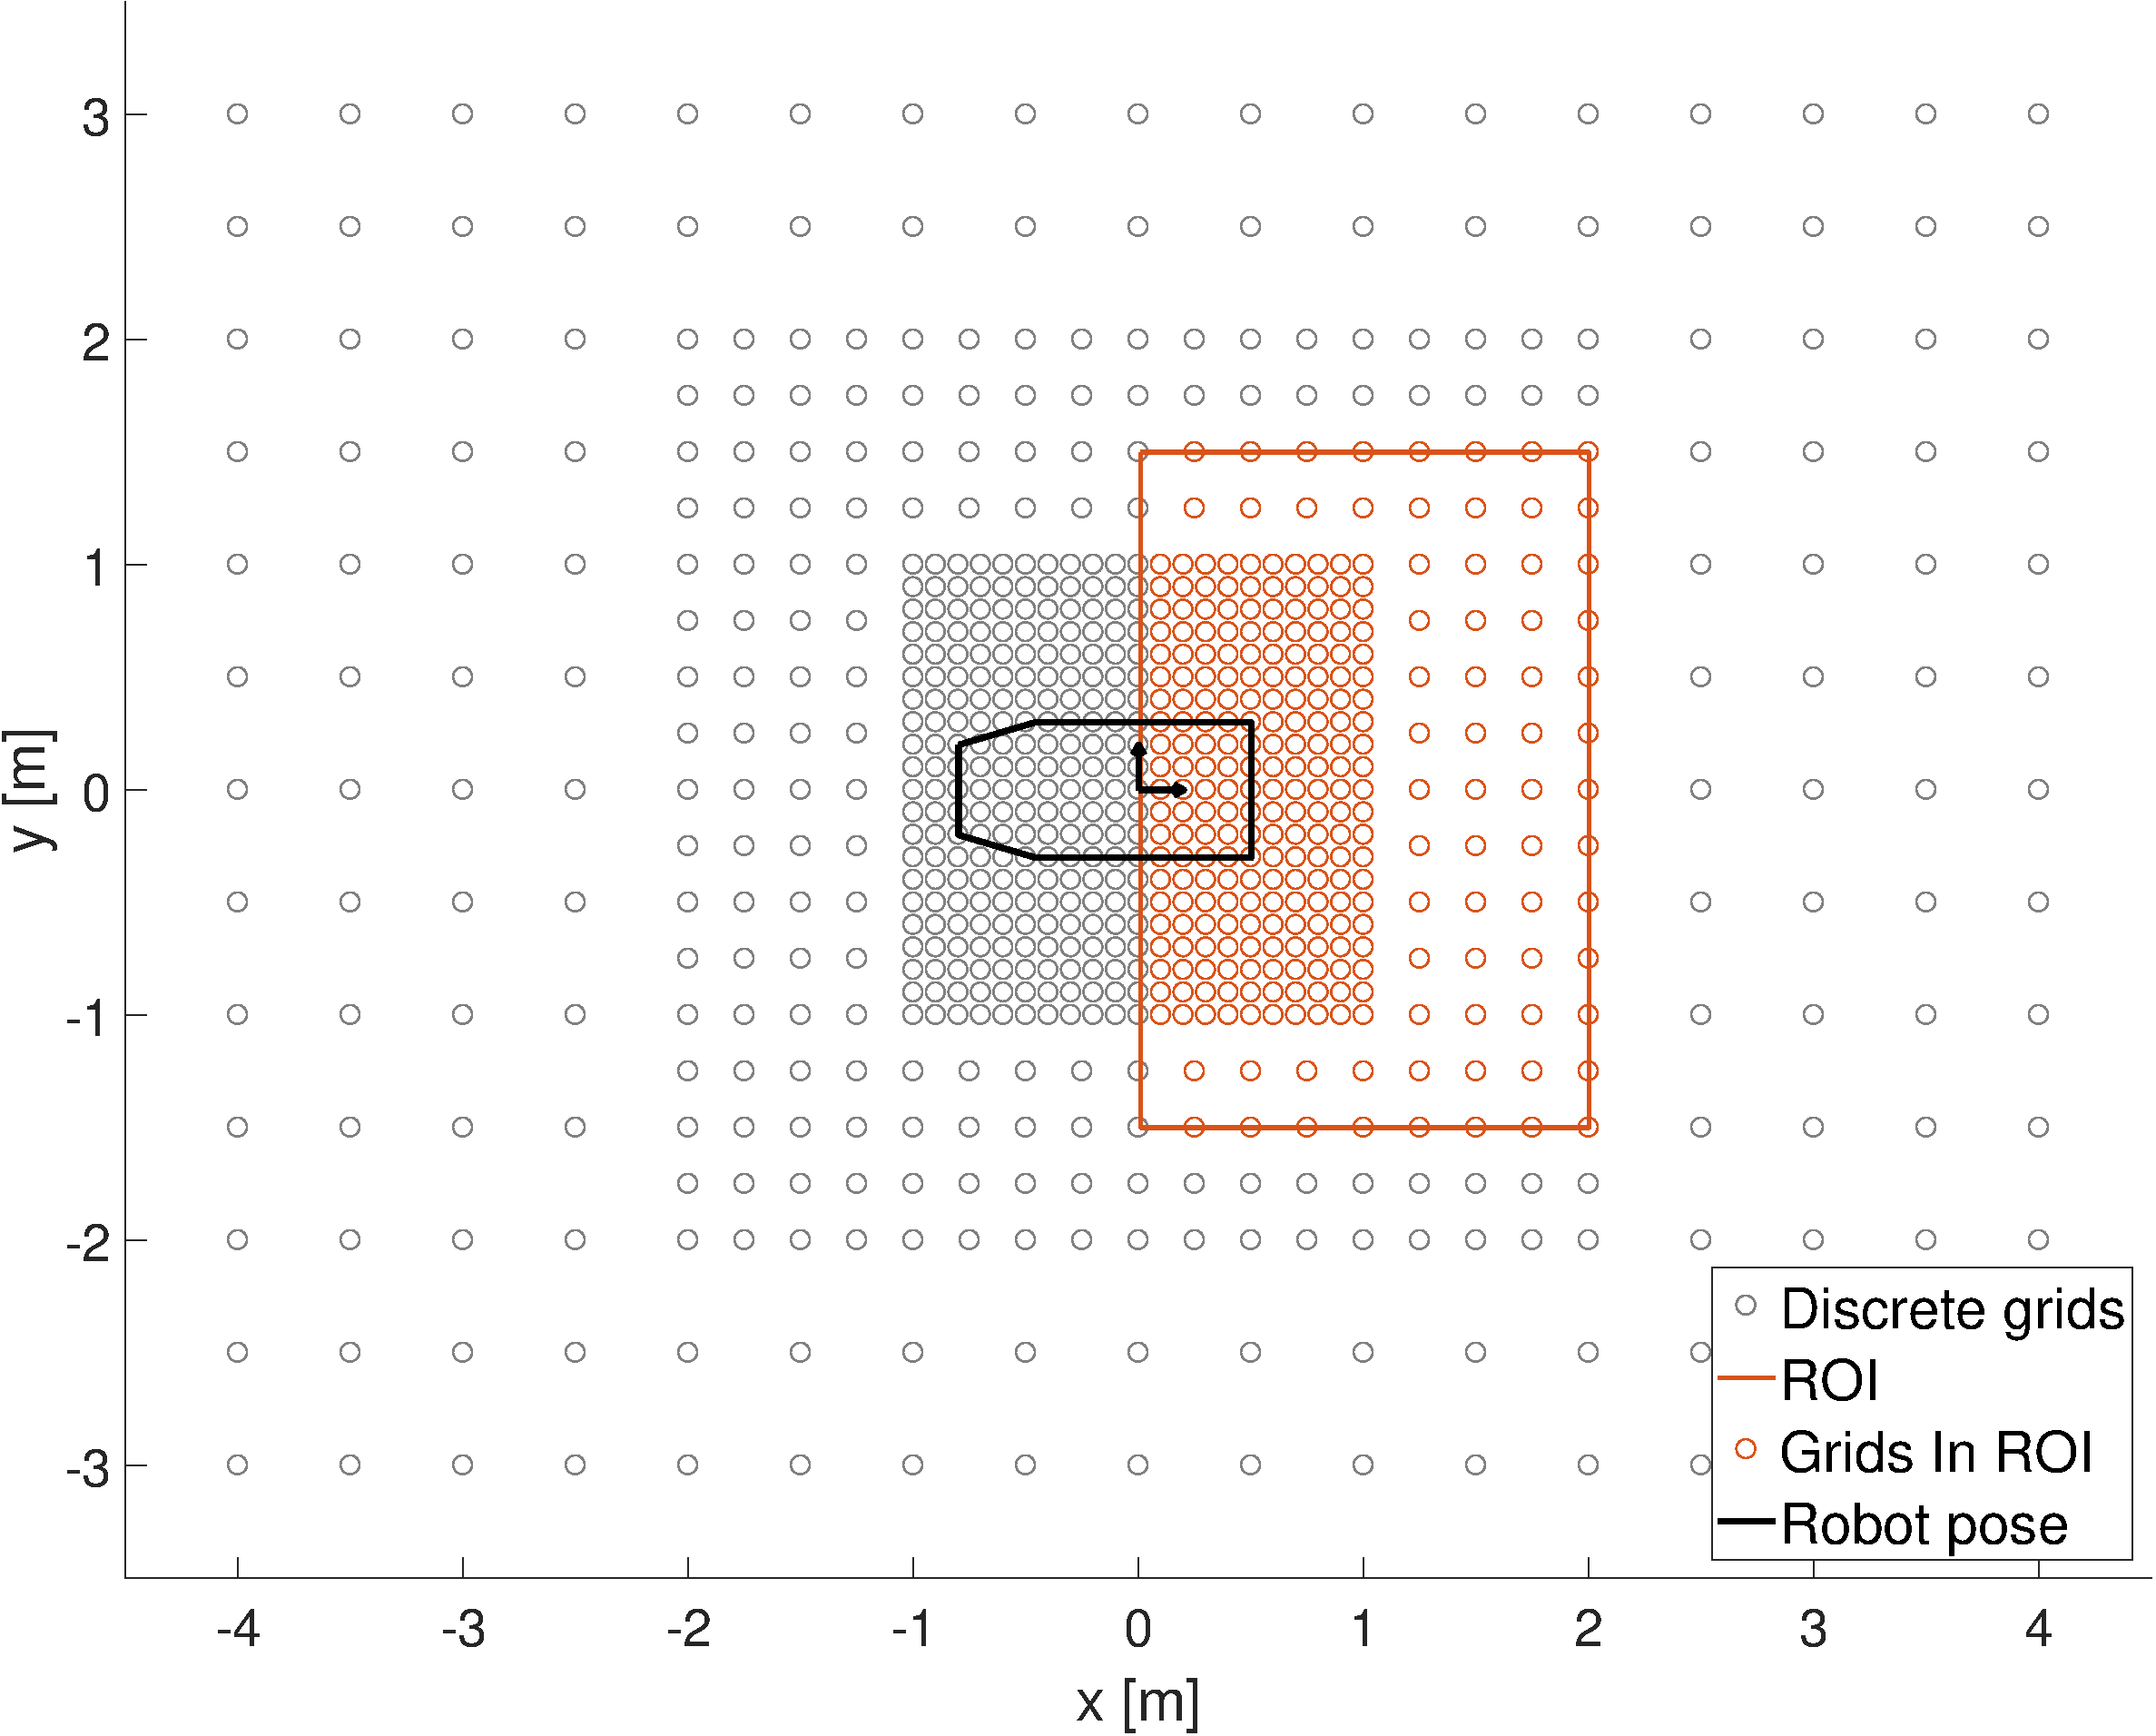
\includegraphics[width=0.90\textwidth]{MultiGirdWithROI.pdf} 
	\doublecaption{MSG and ROI shown at the origin.}{Three different grid sizes are used to sample the environment. Grid cells in the ROI become CEPs, which will be connected to the origin by a geometrical curve. Parameter values are shown in \cref{tab:LSLParVal}. Only feasible trajectories will be added to the set of MPs.\label{fig:MultiGirdWithROI}}
\end{figure}

\begin{table}[!htbp]
\centering
\doublecaption{LSL parameters and corresponding values.}{\label{tab:LSLParVal}}
\vspace{0.2cm}
\begin{tabular}{ r | l | l}
parameter							& 		value			& description	\\ \hline \hline
$dx_1,dy_1$ 						& 		0.10 m 		& Discretization of the fine grid.	\\ \hline
$x_{1,max},y_{1,max}$ 	& 		1.00 m		& Width and height of the fine grid.	\\ \hline
$dx_2,dy_2$ 						& 		0.25 m 		& Discretization of the medium grid.	\\ \hline
$x_{2,max},y_{2,max}$		&		2.00 m		& Width and heigh of the medium grid. \\ \hline
$dx_3,dy_3$ 						& 		0.50 m 		& Discretization of the coarse grid.	\\ \hline
$x_{3,max}$ 						& 		4.00 m		& Width of the coarse grid.	\\ \hline
$y_{3,max}$ 						& 		3.00 m		& Height of the coarse grid.	\\ \hline
$d\theta$							& 		$\pi$/8 rad	& Angular discretization, constant over the whole grid	\\ \hline
$x_{ROI}$ 							&		2.00 m 		& x-distance (only +) defining the ROI.	\\ \hline
$y_{ROI}$							& 		1.50 m		& y-distance (+/-) defining the ROI. 		\\ \hline
$\kappa_{max}$ 				& 		1 m$ ^{-1}$	& Maximum allowed curvature.		 \\ \hline 	
$dx_{EP}$							&		0.50 m		& Manhattan Distance ($\bm{\ell_1}$-norm) between EPs \\ \hline
$res_{OG}$						&		2 cm			& Resolution of the OG\\ \hline 
$res_{path}$						&		1 cm			& Resolution of the path
\end{tabular}
\end{table}
\newpage

\subsection{Motion Primitives Geometry} \label{sec:MPG}
Once the CEPs around the origin are determined, a geometrical connection has to be established between the two robot states. Two possible curve formulations are discussed below, Bézier curves and clothoids. Both have interesting properties to become the basis for the MPs. At the end of this section, the selection of the clothoid will be advocated.

\subsubsection{Bézier curve}
The general form of a Bézier curve of order $n-1$ is shown in \cref{eq:BezierCurveGeneral}. The basis of this curve consists of the Bernstein polynomials, which is the multiplication of the binomial and polynomial coefficients. This is then multiplied by a certain weight, corresponding to the $i^{th}$ control point $P_i$. $n$ represents the amount of control points used to define the Bézier curve \cite{Sederberg2016}.

\begin{equation} \label{eq:BezierCurveGeneral}
\bm{B}(n,u) = \sum_{i=0}^{n-1}
\underbrace{ \begin{pmatrix} n-1 \\ i \end{pmatrix}}_\text{binomial term} \cdot~
\underbrace{(1-u)^{n-1-i} \cdot u^i}_\text{polynomial term}
\cdot~\underbrace{ P_i}_\text{control point}
\end{equation}
Bézier curves are commonly used in Computer Aided Geometric Design Software and are also used in path planning algorithms for mobile robots \cite{PanEtAl2012,ChoiEtAl2008,ChoiEtAl2010}. This is due to the curve’s following interesting properties, also illustrated in \cref{fig:MP_BezierExample}:
\vspace{1em}
\begin{enumerate}
\item The curve passes through the first ($P_1$) and last control point ($P_n$)
\item The curve is tangent to the line connecting $P_1-P_2$ and $P_{n-1}-P_n$
\item The curve lies within the convex hull defined by the $n$ control points.
\end{enumerate}
\vspace{1em}

The problem of connecting one pose to another is mathematically described as a two point G1 Hermite interpolation \cite{WaltonMeek2009}. Due to the first and second property of the Bézier curve, it is possible to explicitly formulate the G1 fitting criterion, by positioning the control points in an adequate way. This is shown for a cubic Bézier curve ($n=4$) in \cref{fig:MP_BezierCubicConstraints}. It is possible to create a path from one arbitrary pose $\bm{p_s}=[x_s, y_s, \theta_s]$ to another $\bm{p_e}=[x_e, y_e, \theta_e]$ while keeping two degrees of freedom: the distance $\norm{P_1-P_2}$ and $\norm{P_3-P_4}$. The shorter this particular distance, the shorter the curve length $L_{tot}$, but the higher the curvature ($\kappa$) of the curve. 

\begin{figure}[!htbp]
	\centering
	\begin{minipage}[b]{.45\linewidth}
		\centering
		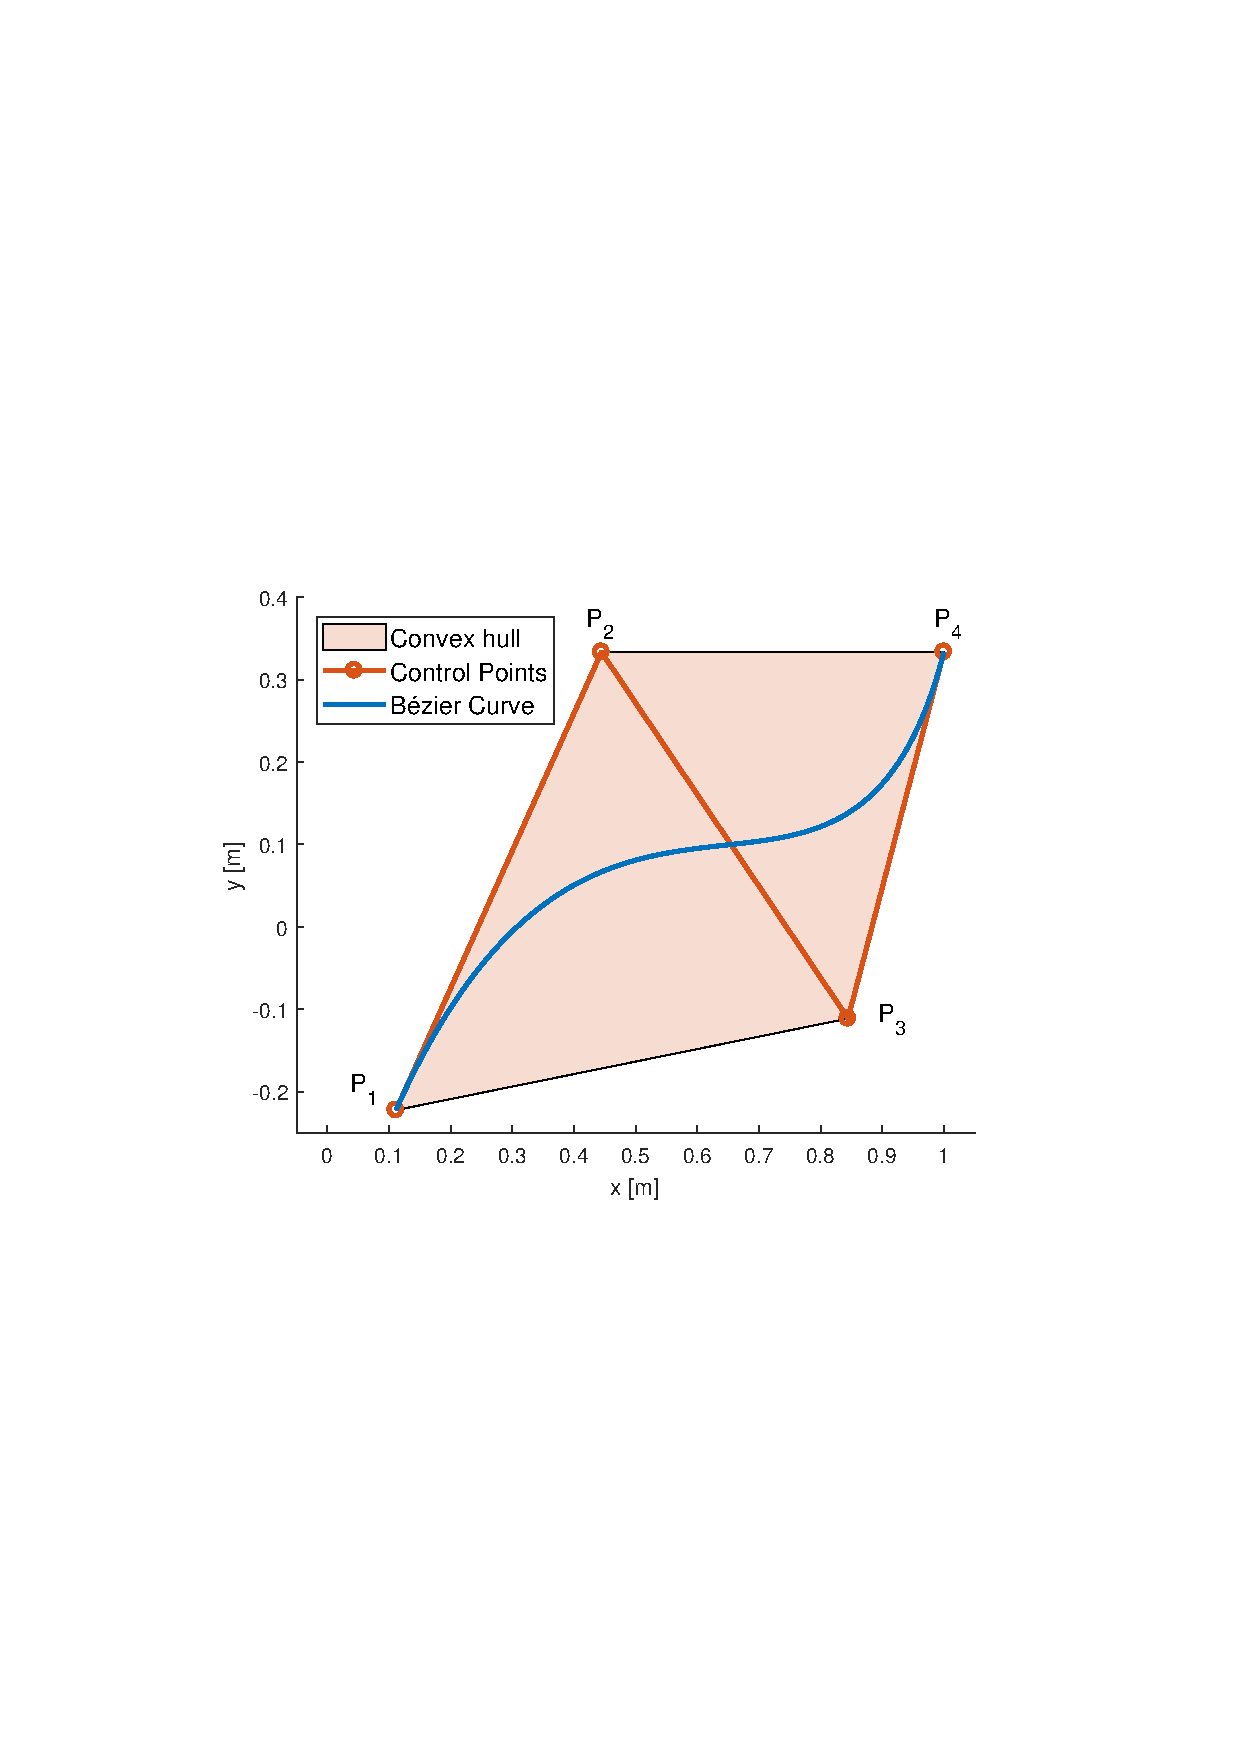
\includegraphics[width=\textwidth]{MP_BezierExample.pdf}
	\end{minipage}
	\hfill
	\centering
	\begin{minipage}[b]{.45\linewidth}
		\centering
		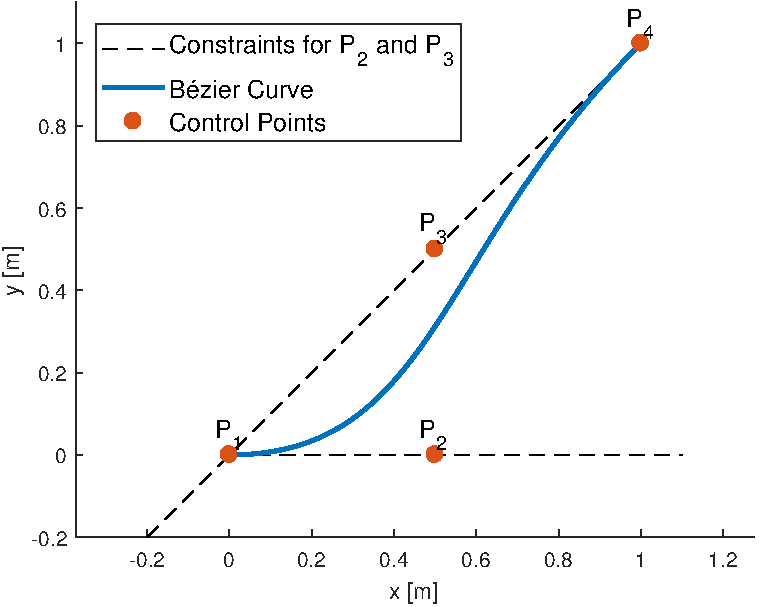
\includegraphics[width=\textwidth]{MP_BezierCubicConstraints.pdf}
	\end{minipage}\\[-7pt]
	\begin{minipage}[t]{.45\linewidth}
		\doublecaption{The 3 primary properties of a Bézier curve.}{A cubic Bézier curve is defined by four control points. It will pass through the first ($P_1$) and last control point ($P_4$), while being tangent to the line connecting $P_1-P_2$ and $P_{n-1}-P_n$ and lying within the convex hull of the four control points.\label{fig:MP_BezierExample}}
	\end{minipage}
	\hfill
	\begin{minipage}[t]{.45\linewidth}
		\doublecaption{G1 fitting with cubic Bézier curves}{is achieved by positioning the two end points on the desired start and end locations and by arranging the two middle points to be tangent to the desired orientations at start and end positions. Two degrees of freedom are left: distance $\norm{P_1-P_2}$ and $\norm{P_3-P_4}$ on that tangent.\label{fig:MP_BezierCubicConstraints}}
	\end{minipage}
\end{figure}

In order to satisfy the constraints presented in \cref{sec:WheelchairPlatform}, a Constrained Optimization Problem (COP) can be formulated in order to generate a particular path. The COP and related equations are furher discussed in \cref{app:BezierCurve}. The objective function of the COP formalized in \cref{eq:BezierCOP} will minimize the bending energy of the curve, resulting in a more comfortable path for the driver \cite{BruyninckxReynaerts1997}, is repeated in \cref{eq:ObjectiveFunction} for convenience. Solving the COP for each CEP yields the set of MPs using a third order ($n=4$) Bézier curve shown in \cref{fig:MPBezierCurve}.

\begin{mini}
{P_{1:4}}{ f(P_{1:4}) = \int_0^1{\kappa(u)^2du}}
{\label{eq:ObjectiveFunction}}{}
\end{mini}

\begin{figure}[!htbp]
	\centering
	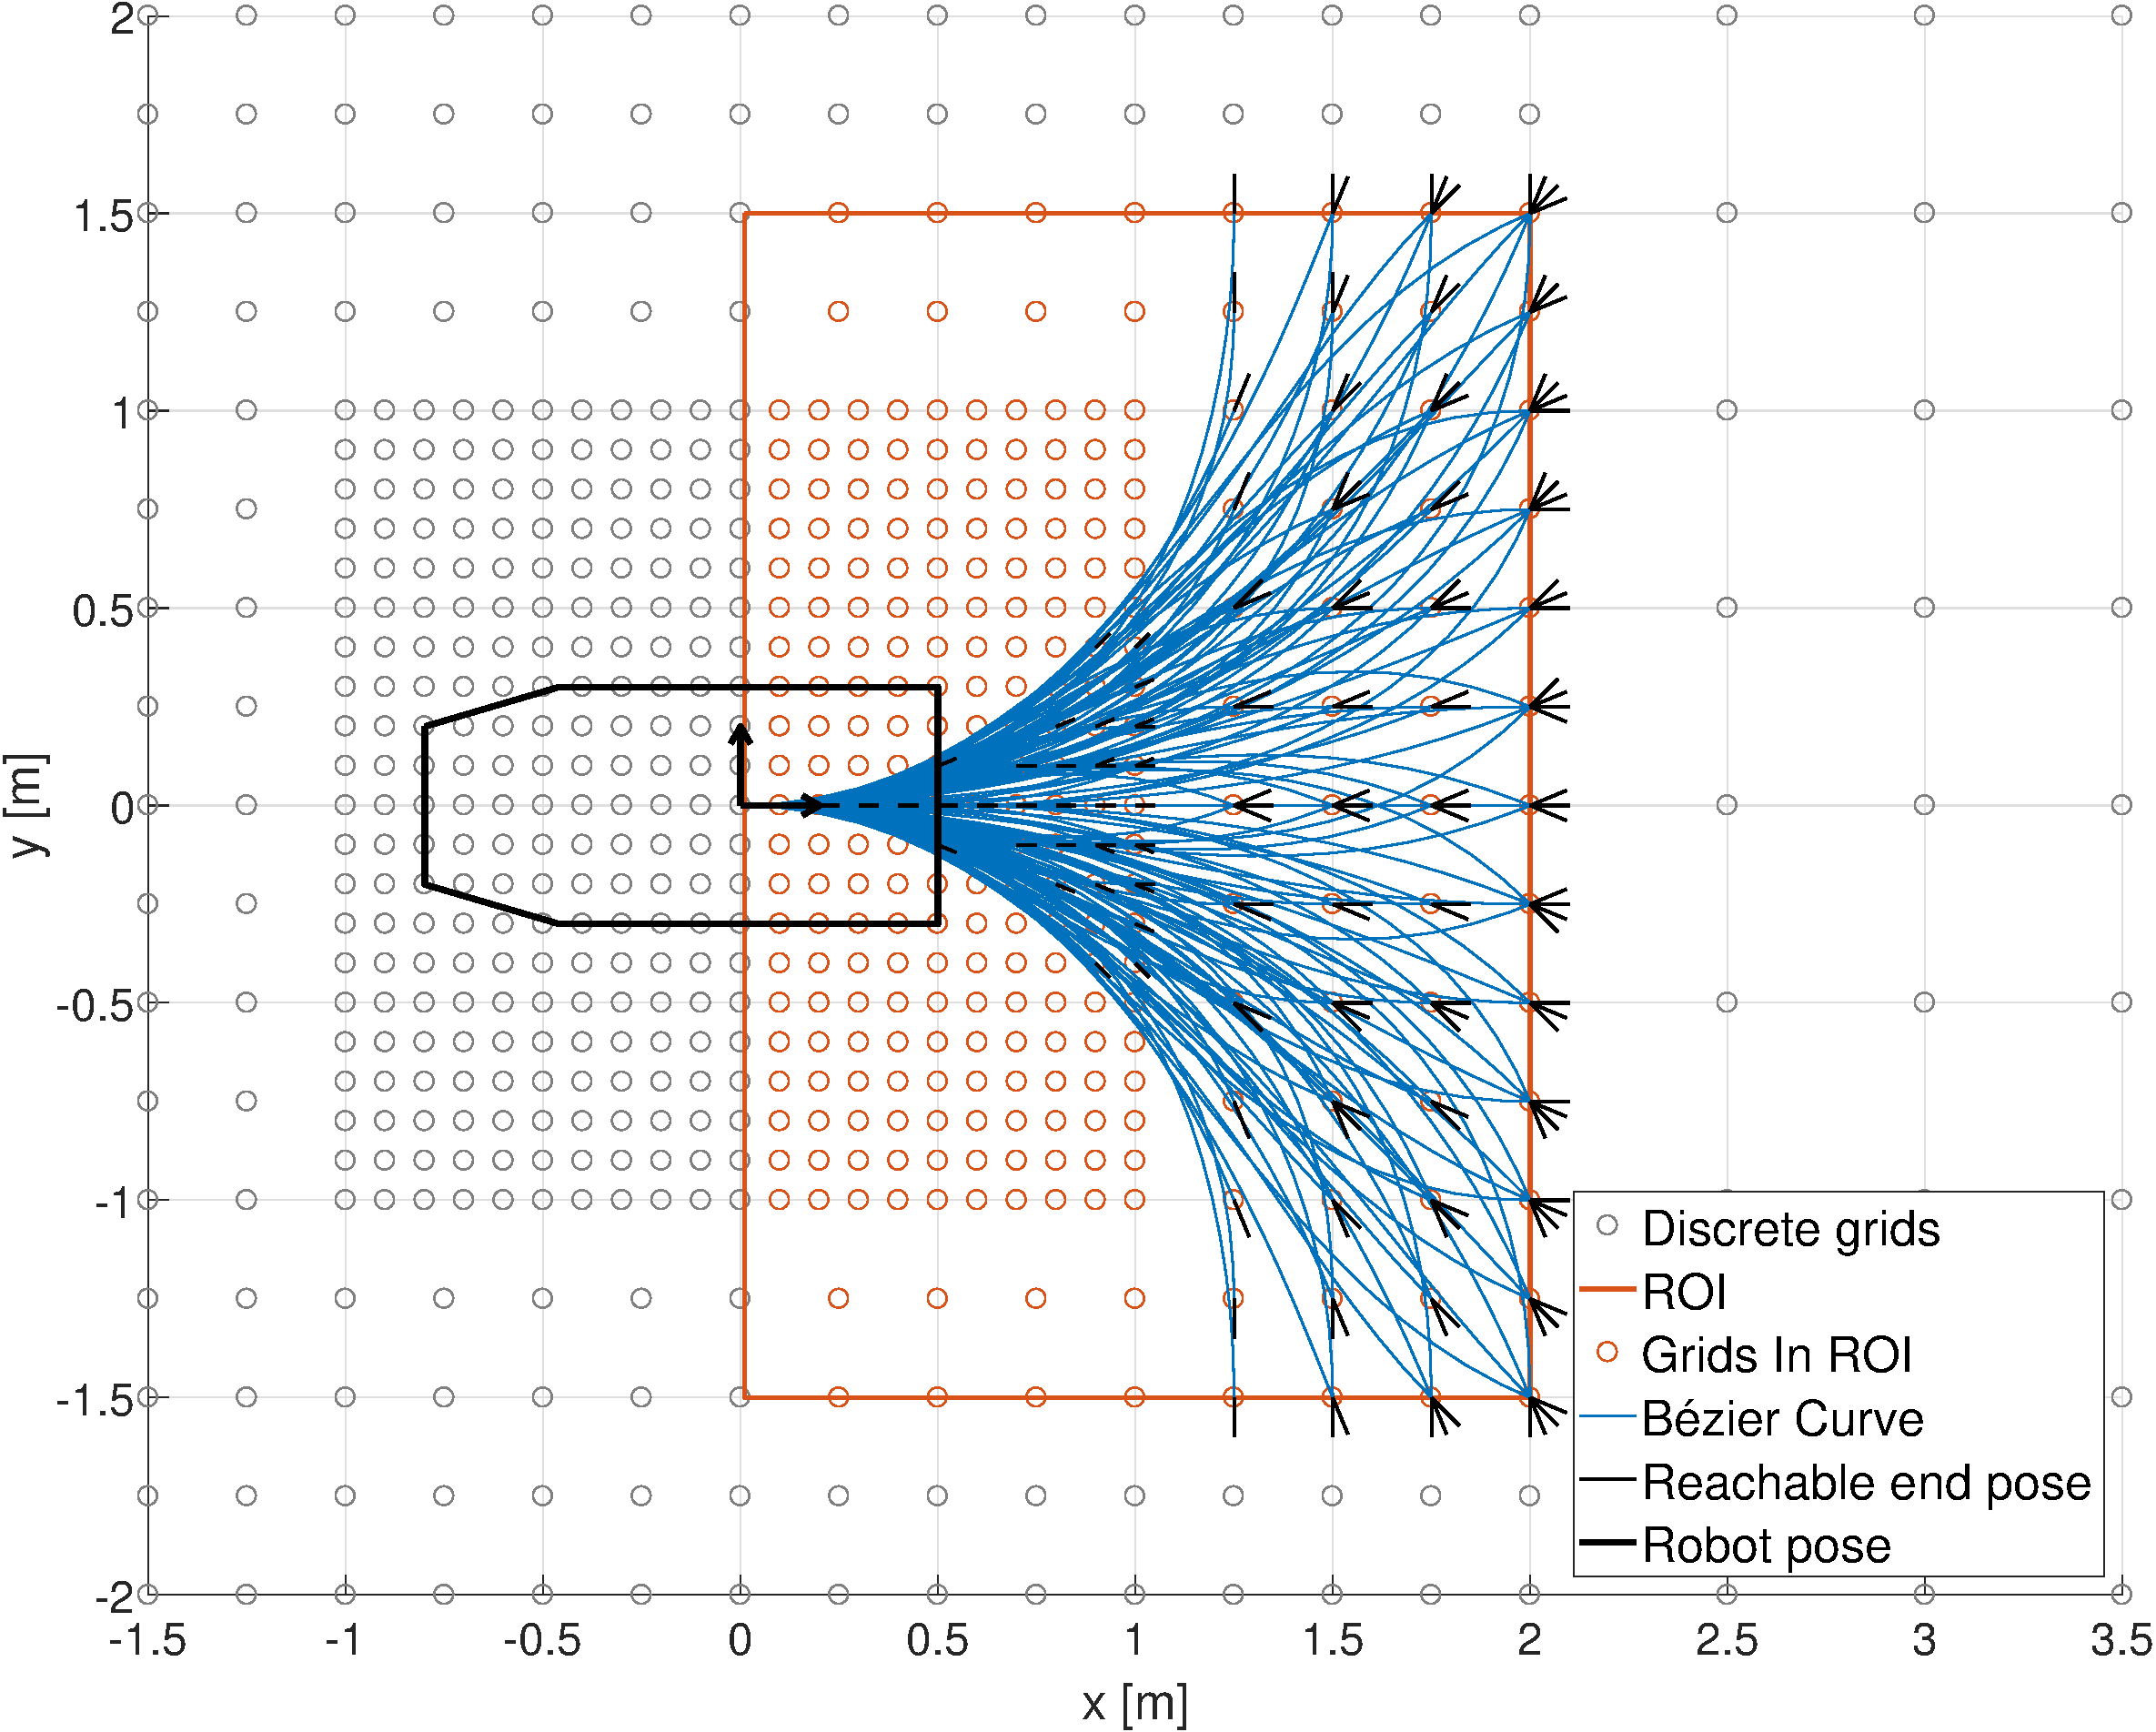
\includegraphics[width=0.85\textwidth]{MPBezierCurve.pdf}
	\doublecaption{Set of MPs based on cubic Bézier curves}{obtained after solving the COP, connecting the origin with feasible states within the ROI.
	\label{fig:MPBezierCurve} }
\end{figure}

\newpage
\subsubsection{Clothoids}
Clothoids (also called Euler or Cornu spirals) are curves whose curvature changes linearly with its arc length \cite{Makino1988}, see \cref{eq:Cloth_kappa}. Clothoids are frequently used for the design of railway tracks \cite{Cope1993} and highway design \cite{Baass1982} to connect a tangent to a circular curve, resulting in a continuous curvature profile. Joining a tangent and a circular curve directly would result in a discontinuity, thus leading to an instantaneous change in the centripetal acceleration, causing discomfort to passengers. Clothoids have also found their application in path planning for mobile robots \cite{FleuryEtAl1995,ScheuerFraichard1997,KellyNagy2003,BrezakPetrovic2011}.

An iterative process has to take place in order to connect one pose $\bm{p_0}$ to another $\bm{p_1}$ using a clothoid, because there is no unique G1 fitting solution (see \cref{fig:Cloth_G1Fitting}). Extensive research has been done to find stable numerical solutions to calculate the Hermite G1 interpolation with a single clothoid curve, which can be formulated as a system of three nonlinear equations (yielding multiple solutions), see \cref{eq:Cloth_dtheta,eq:Cloth_dx,eq:Cloth_dy}. Walton and Meek \cite{WaltonMeek2009} designed their algorithm to handle three different situations, straight lines, circles and clothoids to then solve only one single nonlinear equation. However, when the solution of a clothoid approaches the shape of a circle ($\kappa'\approx0$) or a straight line ($\kappa = \kappa' \approx 0$) the root of the nonlinear equation becomes ill-conditioned, resulting in numerical errors. In \cite{BertolazziFrego2015} this problem is solved by recasting the problem into a well-conditioned zero of a unique nonlinear equation. Moreover, their algorithm does not treat straight lines, circles and clothoids differently and thus achieves robust results at the transition zones. Their source code is available online \cite{BertolazziFrego2016} and has been used without modification to generate the clothoids.

\begin{figure}[!htbp]
\centering
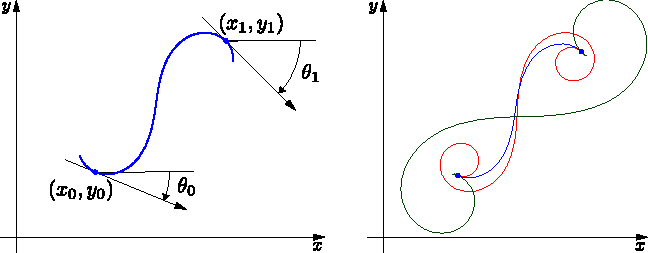
\includegraphics[width=0.85\textwidth]{Cloth_G1Fitting.pdf}
\doublecaption{(left) Notation for the G1 Hermite interpolation scheme (right) yielding multiple solutions using clothoids}{(from \cite{BertolazziFrego2015}).\label{fig:Cloth_G1Fitting}}
\end{figure}

By applying G1 interpolation, the smooth transition of curvatures is not guaranteed; this would require G2 Hermite interpolation. G2 fitting would result in a smoother curve but will be computationally more expensive due to additional constraints. As G1 continuity is acceptable for this application, G2 is not applied. If G2 continuity is preferred, e.g. for the generation of local paths for car-like vehicles, the use of piecewise clothoid curves is necessary, which has been developed in \cite{McCraeSingh2009}.

Solving the 2 point Hermite interpolation for each CEP with clothoids yielding a feasible path forms the set of MPs shown in \cref{fig:MPClothoid}.

\begin{align}
\kappa(s)&=\kappa's + \kappa_0,	& \kappa' &, \text{change of curvature, constant} \label{eq:Cloth_kappa} \\ 
\theta'(s)&=\kappa(s),						& \theta(0)&=\theta_0	& \theta(l)&=\theta_1 \label{eq:Cloth_dtheta} & \\
x'(s)&=\cos\theta(s), 							& x(0)&=x_0 					& x(l)&=x_1 \label{eq:Cloth_dx} \\
y'(s)&=\sin\theta(s), 							& y(0)&=y_0 					& y(l)&=y_1 \label{eq:Cloth_dy} 
\end{align}

\begin{figure}[!htbp]
\centering
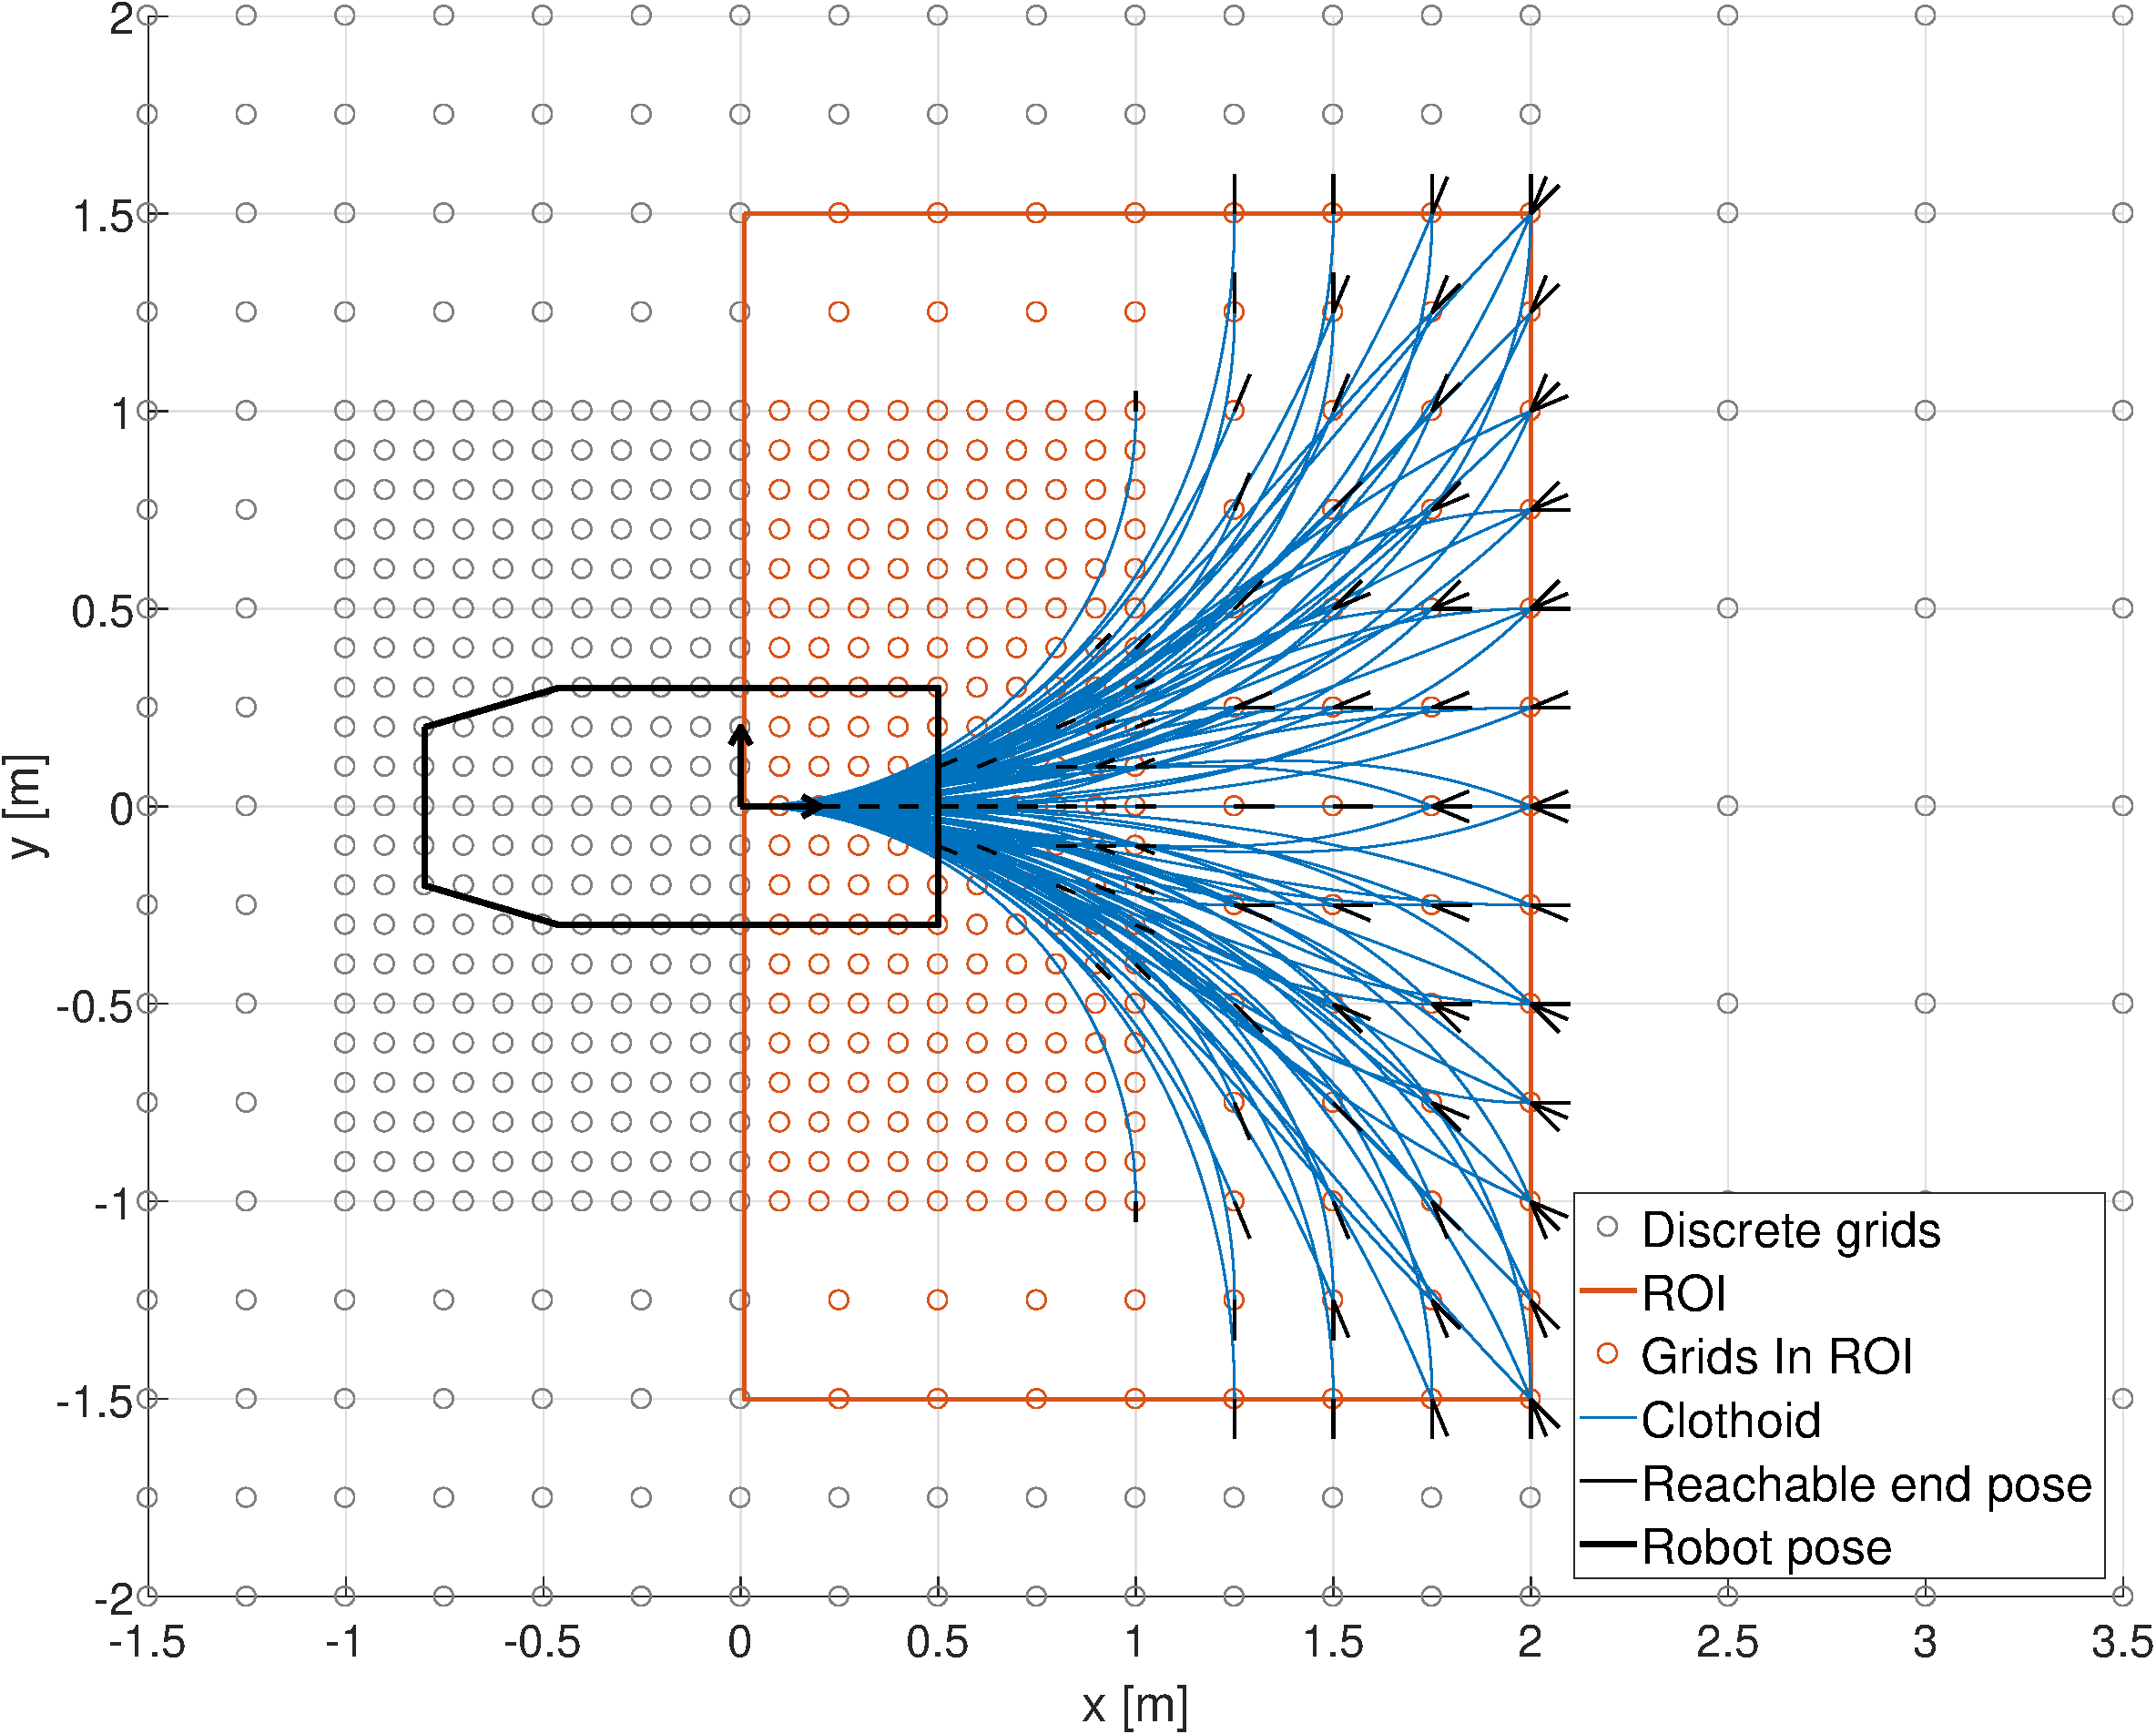
\includegraphics[width=\textwidth]{MPClothoid.pdf}
\doublecaption{Set of MPs based on clothoids}{calculated with \cite{BertolazziFrego2016}, connecting the origin with feasible states within the ROI.
\label{fig:MPClothoid}}
\end{figure}

\subsubsection{Selected Motion Primitive}
A first criterion for the selection of the MP could be to look at the diversity that each primitive offers. When looking at the unique states that each curve can reach, shown in \cref{fig:MPDifference}, it is clear that the formulation of the Bézier curve imposes fewer restrictions than the clothoid.

\begin{figure}[!htbp]
	\centering
	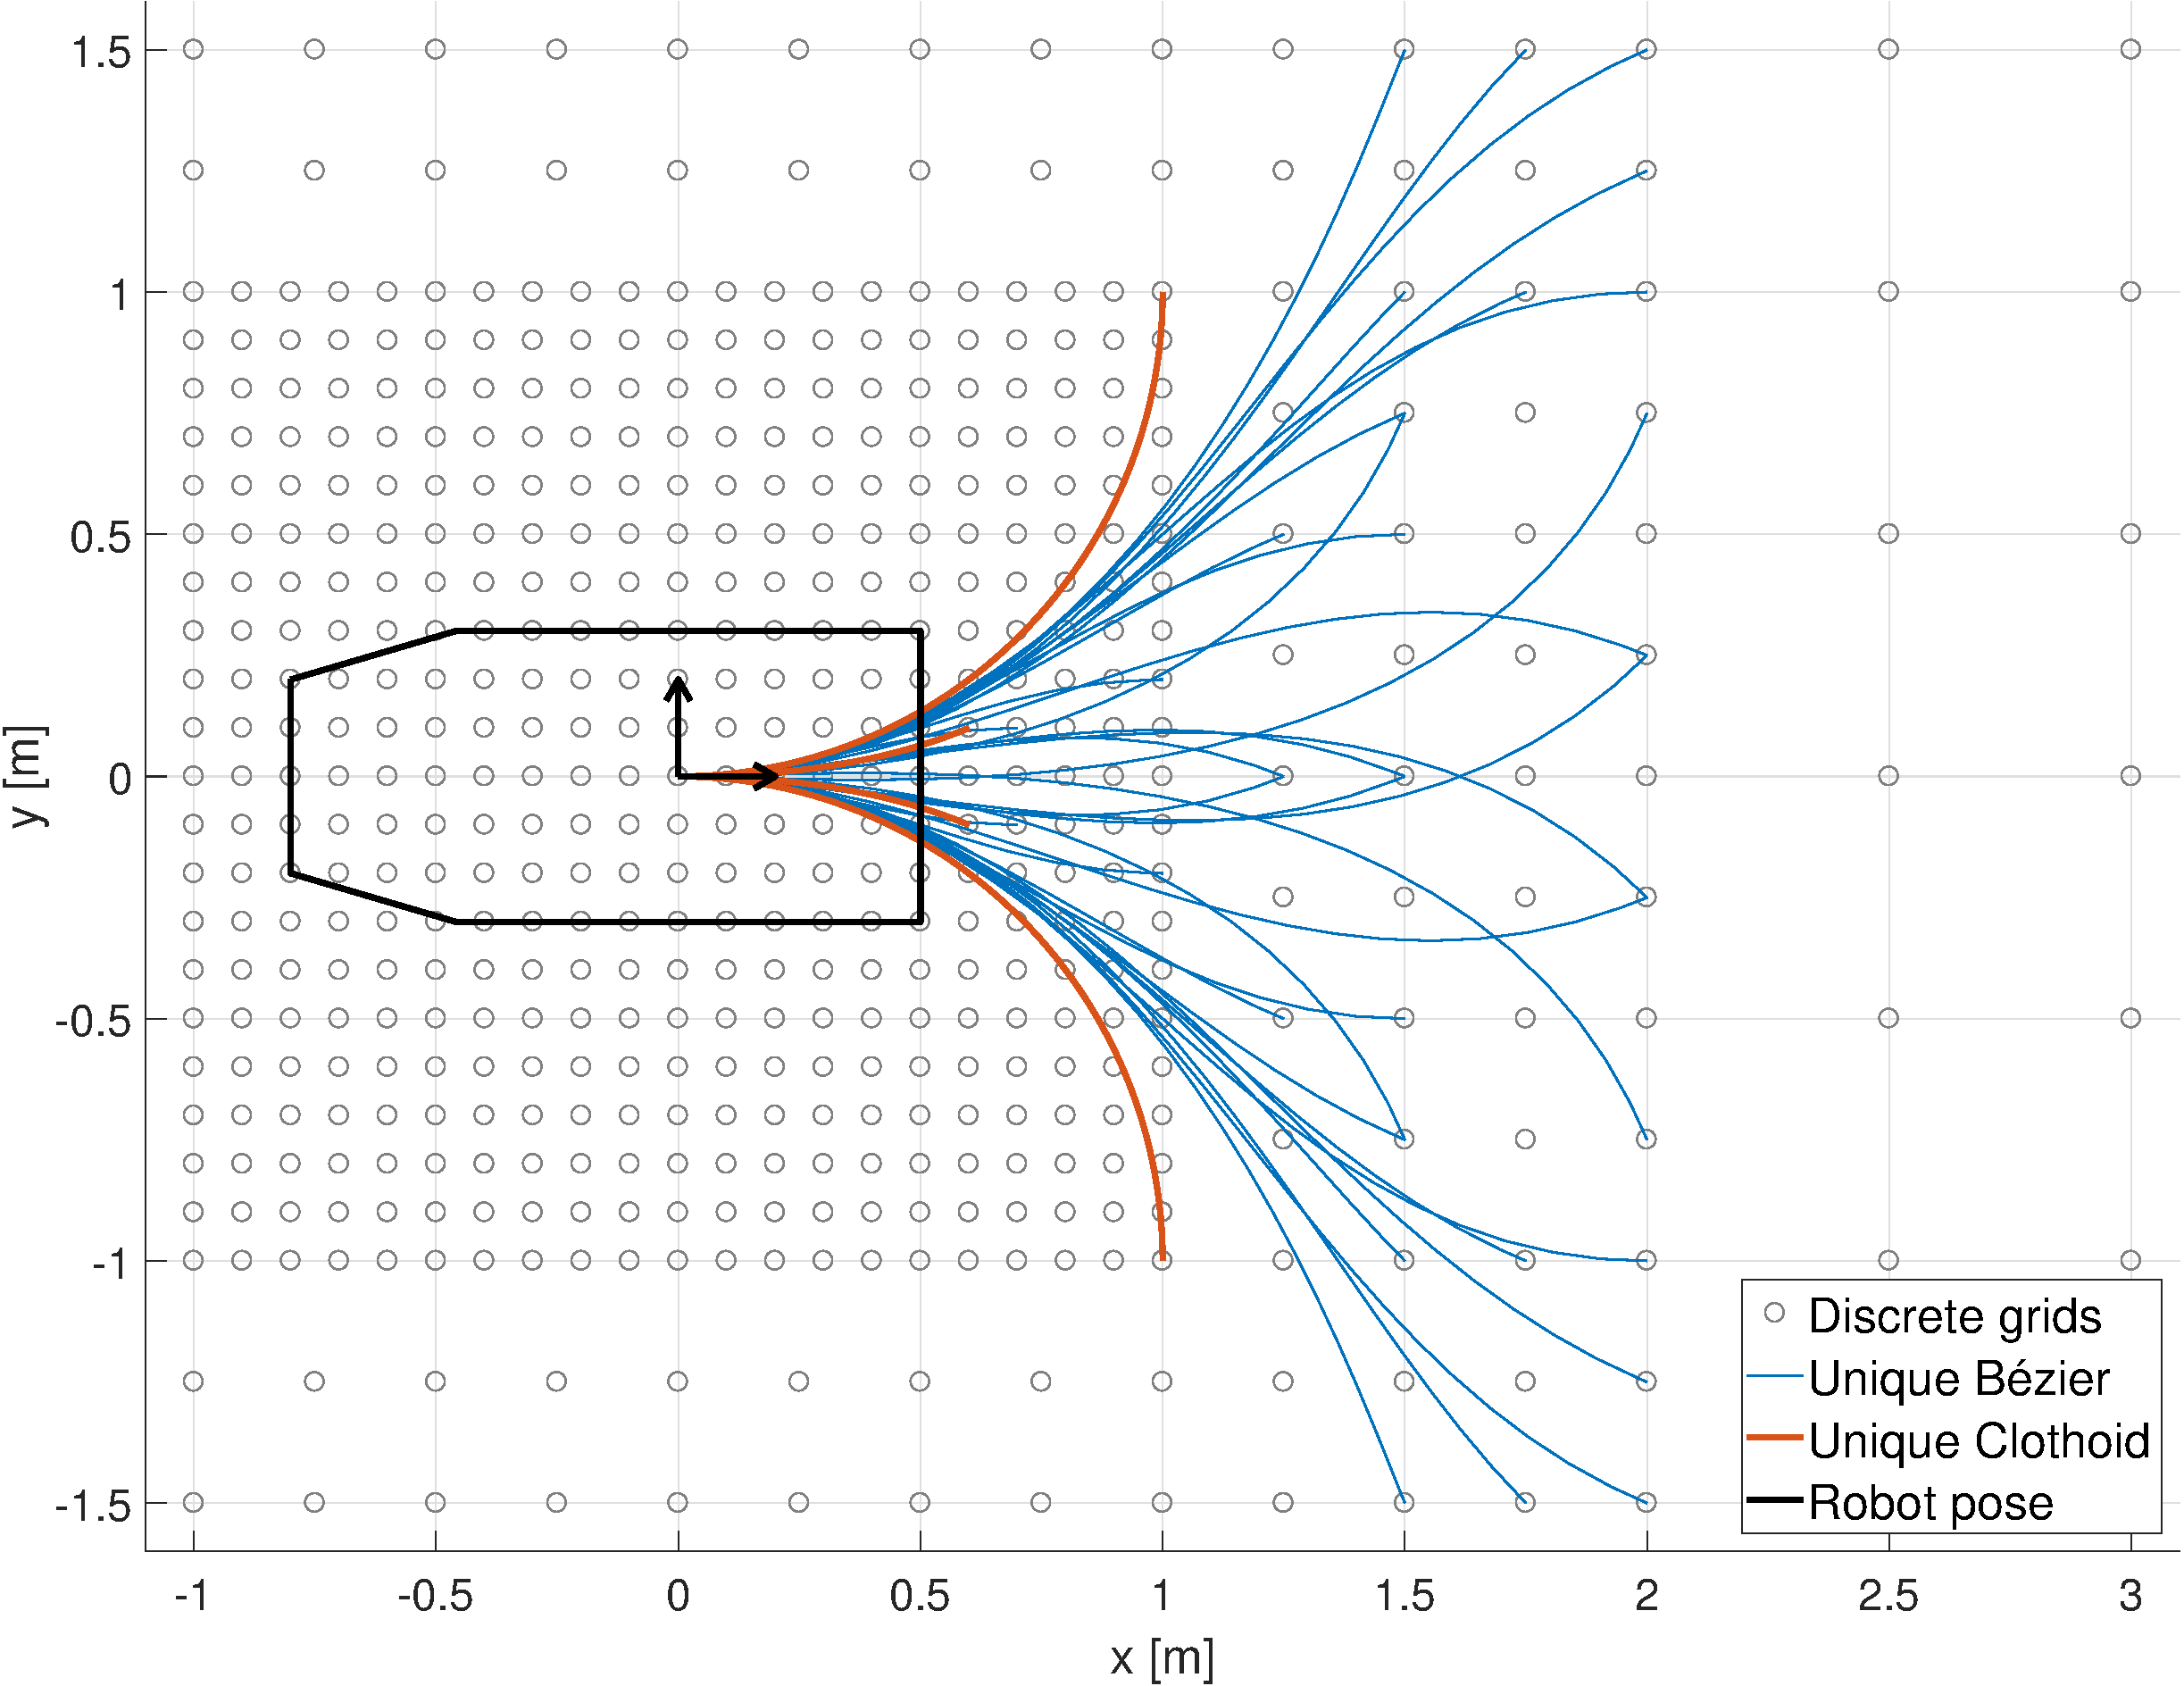
\includegraphics[width=0.7\textwidth]{MPDifference.pdf}
	\doublecaption{Unique end poses achieved by the two different curves.}{The Bézier curve has clearly a less restrictive formulation resulting in more unique end poses compared to the clothoid. However, this does not imply that it is therefore a better basis for the MP.
	\label{fig:MPDifference}}
\end{figure}

Even though the designed path planner focuses on the geometry of the curve, it is still relevant to consider the control actions (right and left wheel rotation speed $u_{right},u_{left}$) the robot should send to its actuators to follow a desired path. Since the sAMR is differentially driven (see \cref{sec:WheelchairPlatform}) and by further assuming a constant linear velocity ($v$), the remaining parameter would be the angular velocity ($\omega$). The latter can in turn be reformulated to the curvature ($\kappa$) of the curve. See \cref{eq:Url2VW,eq:IRC,eq:omegaKappa,eq:VKappa2UrUl} for a full derivation. 

\begin{align}
v &= \frac{r_{wheel}\cdot(u_{right} + u_{left})}{2} & \omega &= \frac{r_{wheel}\cdot(u_{right} - u_{left})}{B} \label{eq:Url2VW} \\
v & = R \cdot \omega & \kappa &= \frac{1}{R} \label{eq:IRC}\\
\omega & \sim \kappa & &\text{if $v$ constant} \label{eq:omegaKappa} \\
u_{right} & = \frac{b\cdot v}{2\cdot r_{wheel}} \kappa + \frac{v}{r_{wheel}} & u_{left} & = \frac{-b \cdot v}{2\cdot r_{wheel}} \kappa + \frac{v}{r_{wheel}} \label{eq:VKappa2UrUl}
\end{align}

\vspace{1em}

The control action will thus be linearly dependent on the curvature while driving at a constant linear speed. This is again a purely geometrical parameter, which has already been calculated for the Bézier curves and clothoids in \cref{eq:curvature,eq:Cloth_kappa} respectively. 
To compare the effort the actuator has to make, the curvature of the Bézier curve and the clothoid are plotted for a common start- to end pose ($[0,0,0\degree] \text{ to } [1.25,1.5,90\degree]$) in \cref{fig:MPCurvatureComp}. 

There is a clear difference between the curvatures of both trajectories in the left figure. The reason why the Bézier curve has this more pronounced curvature profile is due to the objective function used in the COP, recall \cref{eq:ObjectiveFunction}. This ``forces'' the curvature to change abruptly in order to minimize the surface obtained after the integration. The path defined by the Bézier curve is therefore more difficult to follow then the path based on the clothoid. A possible solution would be to change the objective function of the COP to the one proposed in \cref{eq:ObjectiveFunctionMod} to minimize the change in curvature. This change of objective function forces the Bézier curve to approximate a clothoid, but is computationally expensive compared to the calculation of a clothoid.

\begin{mini}
{P_{1:4}}{ f(P_{1:4}) = \int_0^1{\kappa'(u)^2du } }
{\label{eq:ObjectiveFunctionMod}}{}
\end{mini}

\begin{figure}[!htbp]
	\centering
	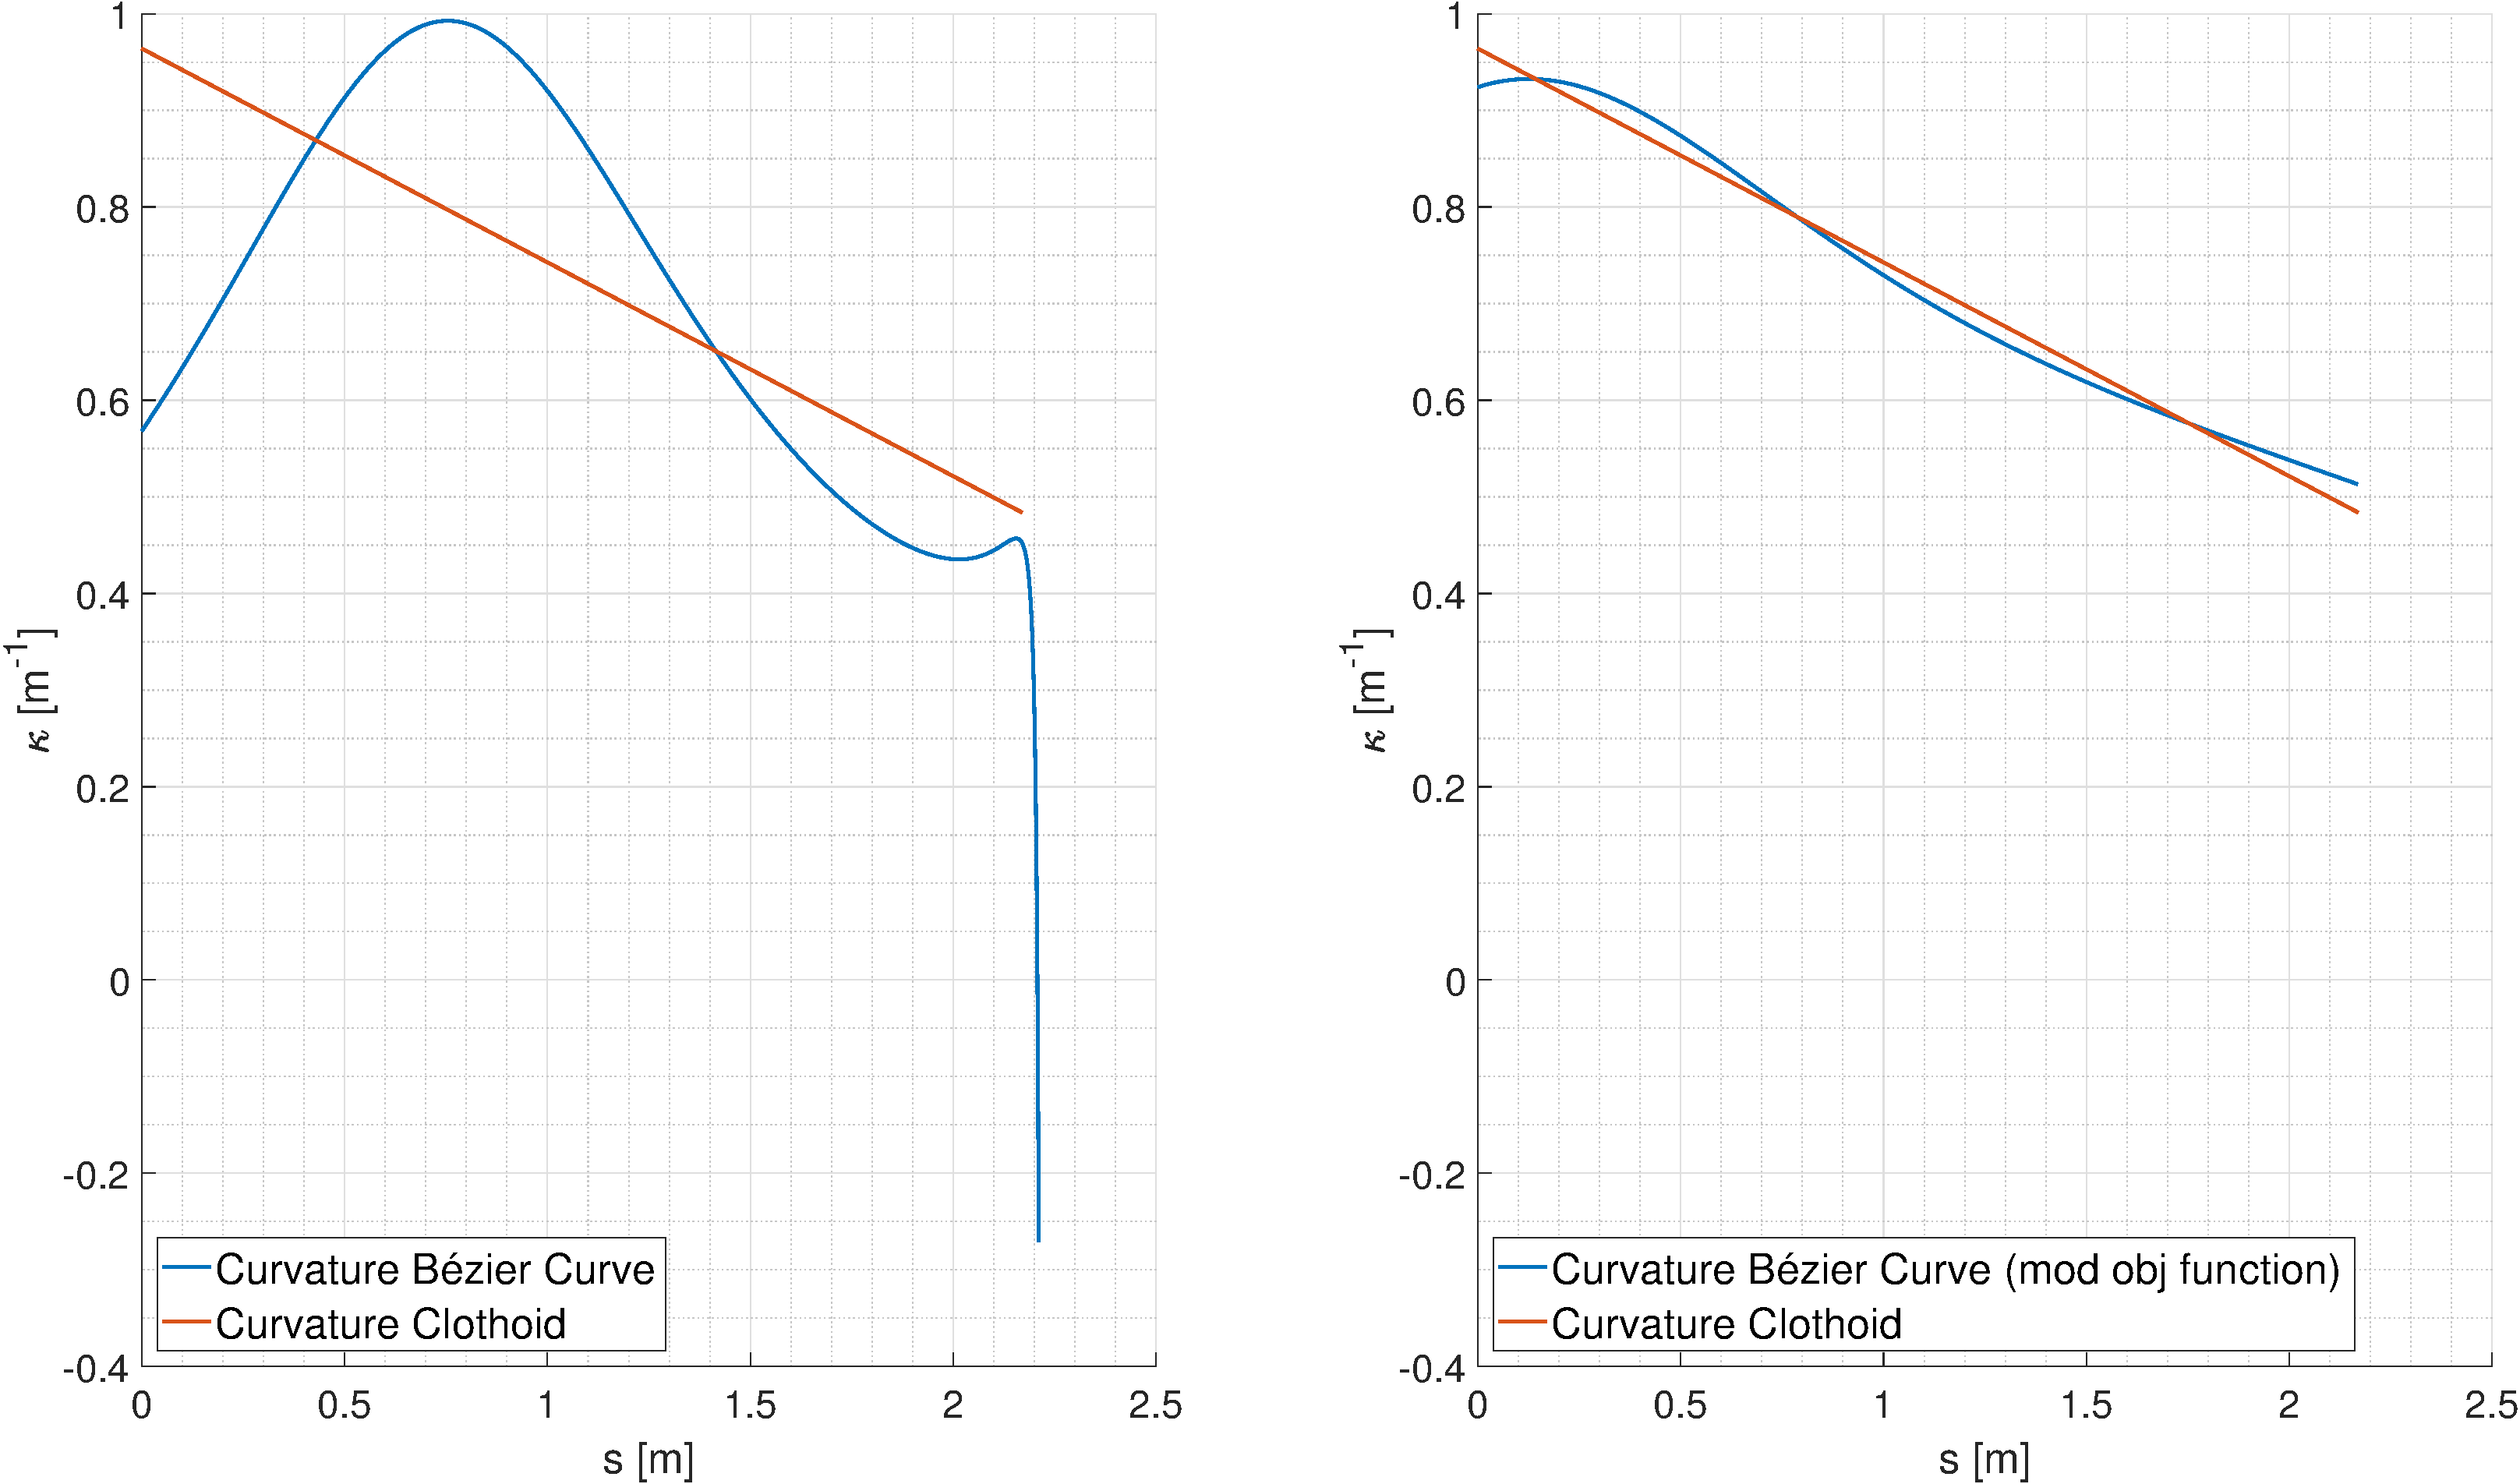
\includegraphics[width=\textwidth]{MPCurvatureComp.pdf}
	\doublecaption{Comparison of the curvature of the 2 types of MP connecting the same start- and end pose.}{(left) The COP based on \cref{eq:ObjectiveFunction} leads to abrupt changes in the curvature resulting in a path that is more demanding to follow compared to the red linear curvature of the clothoid. (right) Adapting the COP objective function to \cref{eq:ObjectiveFunctionMod} would result in a Bézier curve that is nearly identical to a clothoid and thus easier to follow.
	\label{fig:MPCurvatureComp}}
\end{figure}

After the above assessment of both types curves, the clothoid is chosen to be used as the basis for the MP. This choice is based on the clothoid’s ideal characteristics when driving at constant speed. The input of the actuator (wheel rotation speed) only has to change linearly. The main disadvantage of the clothoid as compared to the Bézier curve is its more restrictive formulation, resulting in less achievable end poses. This problem will be addresses in the next section.

\subsection{Expansion Position} \label{sec:EP}
\begin{figure}[!htbp]
	\centering
	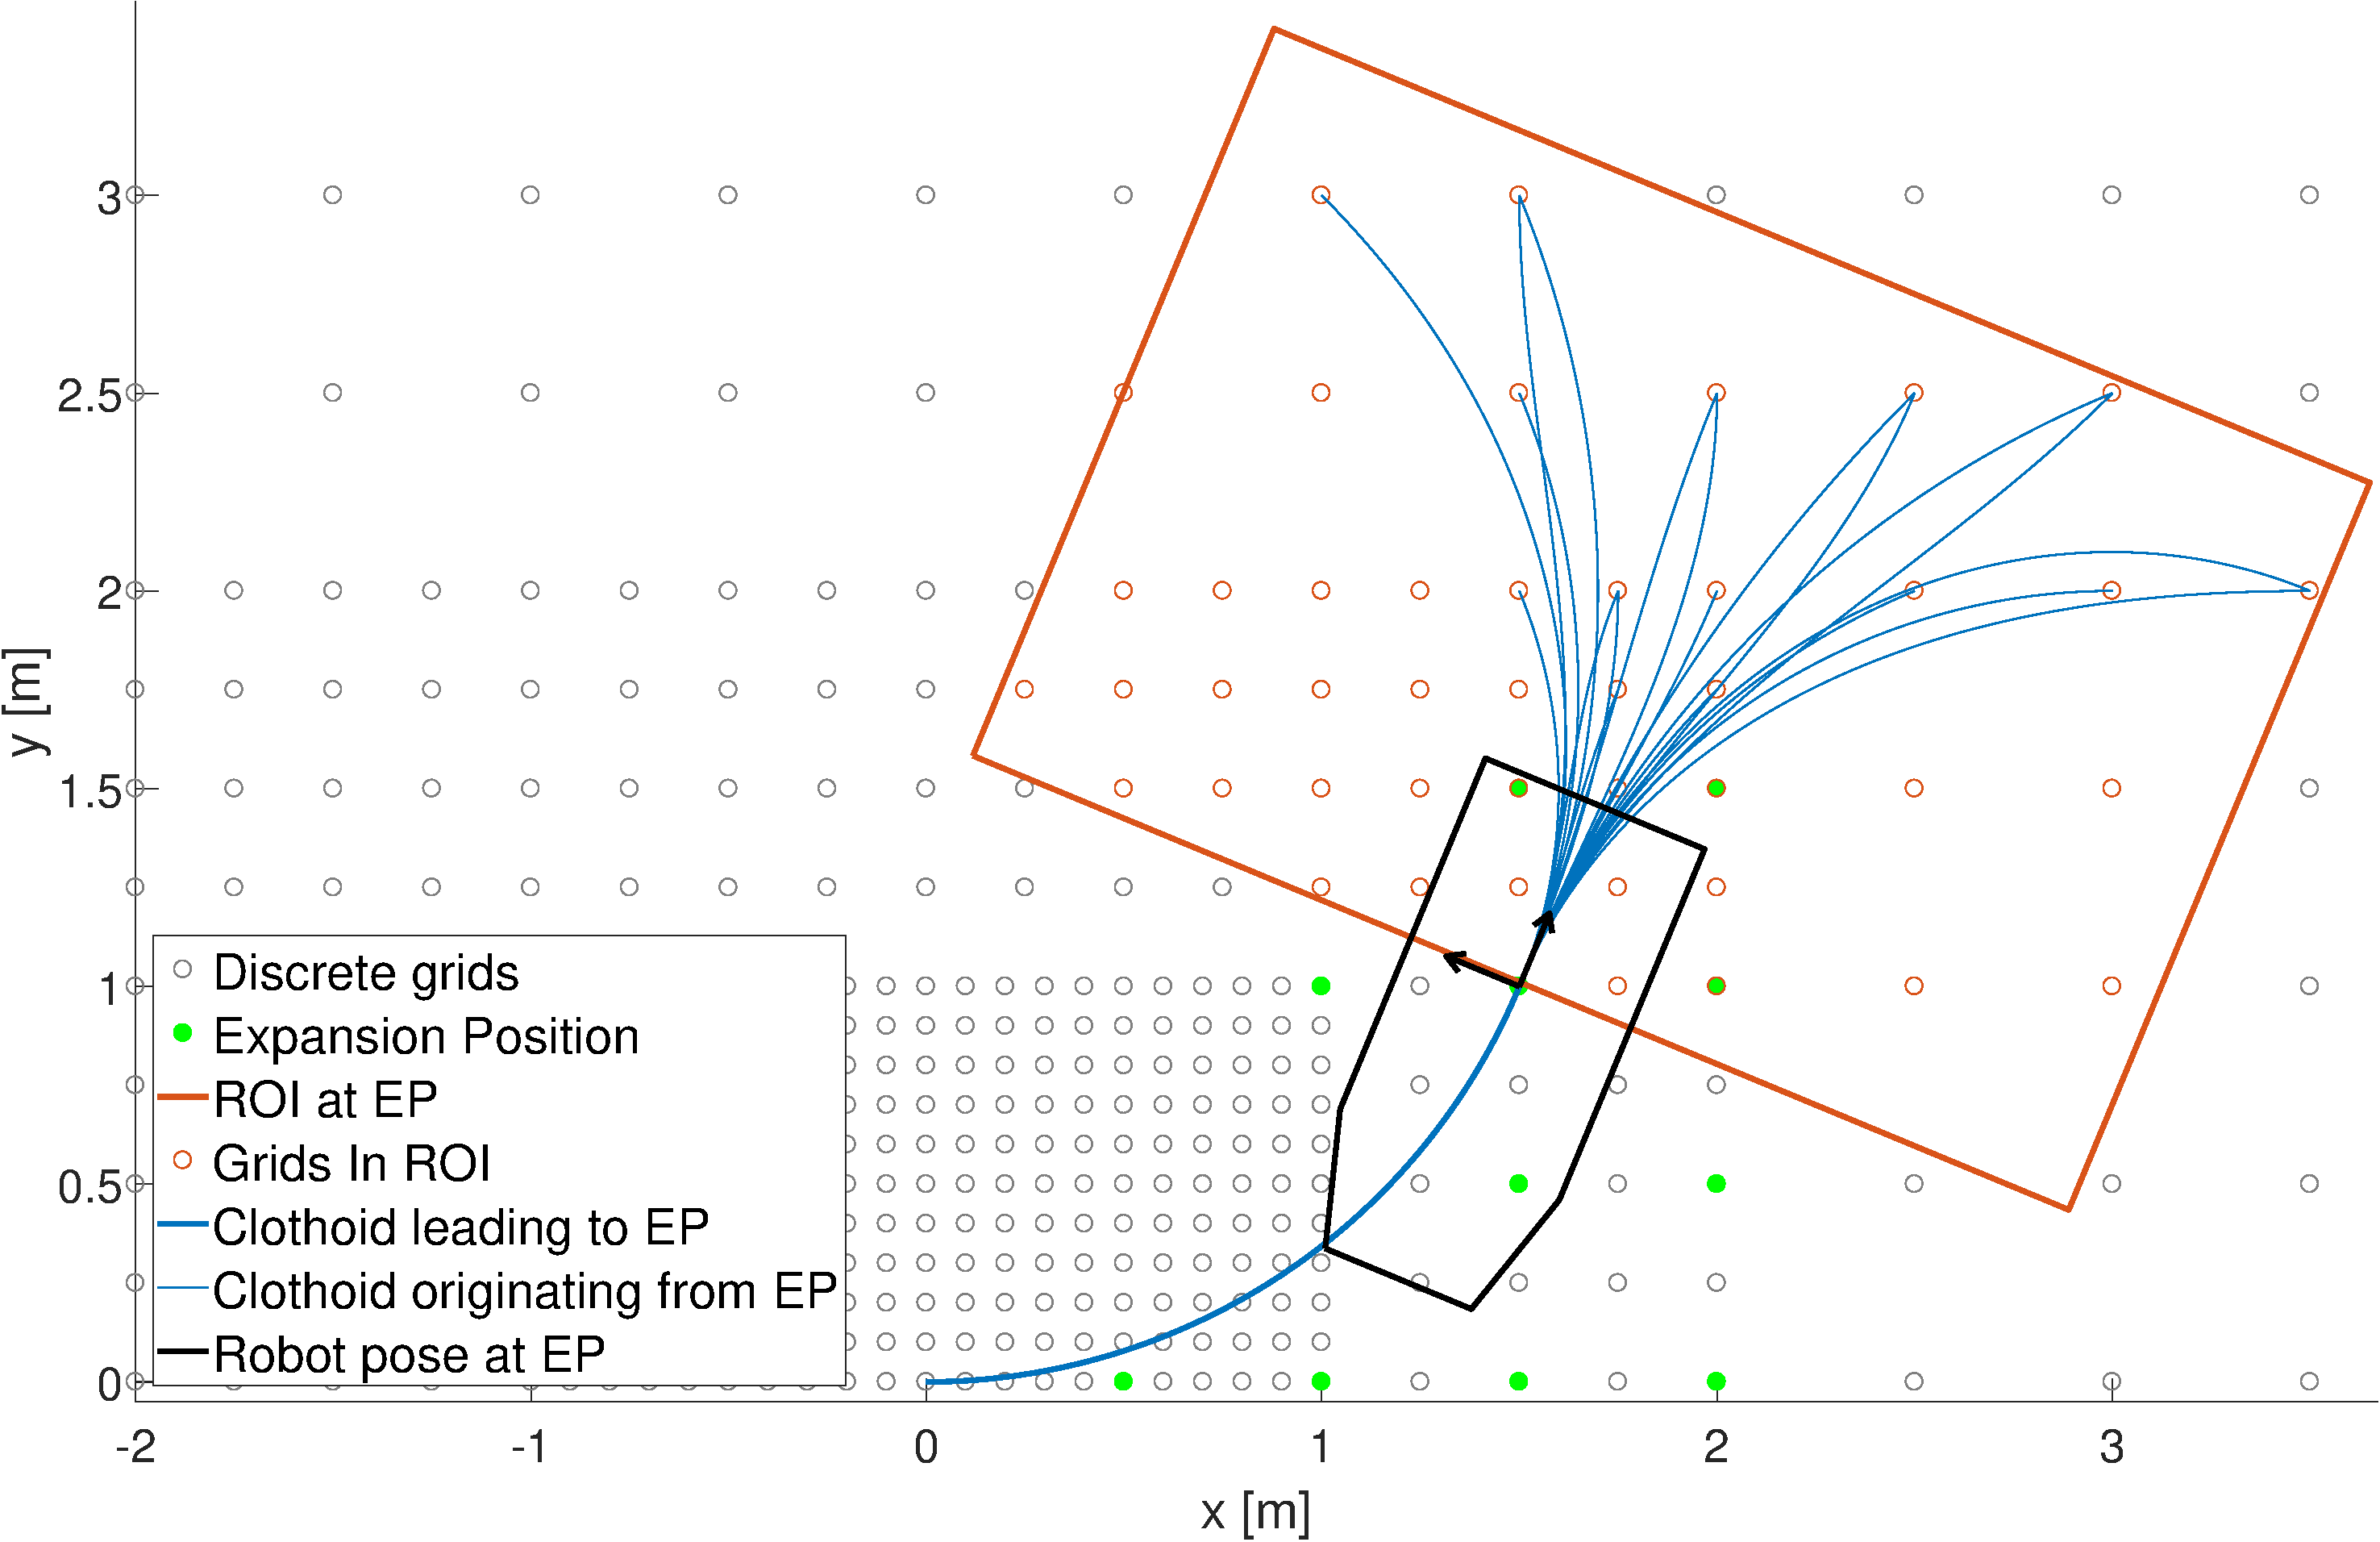
\includegraphics[width=\textwidth]{MultiGirdWithEPROI.pdf}
	\doublecaption{Example of the EP and ROI}{at $[1.5,1,45 \degree ]$. CEPs are now linked with the pose that the robot would have at that EP and not with the origin.\label{fig:MultiGirdWithEPROI}}
\end{figure}
%CHANGED
% “ Note that those discrete poses..." to “Remark”
Finally, in order to propose a lager variety of paths, the procedure of connecting CEPs to the set of MPs is repeated at certain discrete positions, called Expansion Positions (EPs). EPs are defined as reachable end poses directly connected to the origin, with a Manhattan Distance ($\bm{\ell_1}$-norm) equal to a multiple of $dx_{EP}$. It should be noted that those discrete poses in the ROI (at that EP) will be connected with the pose at that EP, and not at the origin. There will be significantly less CEPs if the EP is further away from the origin, due to the use of the MSG, thereby reducing the number of paths leading far away from the origin. An example of this procedure is shown in \cref{fig:MultiGirdWithEPROI}.

Repeating this for every EP results in a LSL, a set of paths is generated starting from the origin and connecting with feasible trajectories, based on clothoids, to reach end poses in the surrounding of the wheelchair. A ``clean-up'' procedure has to be performed to eliminate paths with start- and end poses that have been achieved previously in the LSL set to obtain a unique set of paths. This is illustrated in \cref{fig:LSLClothoid}. Backwards driving and on-the-spot-turning are not shown. An overview of the algorithm of this section is provided in \cref{alg:LSL}. The output of this algorithm is the LSL data structure ($\mathcal{LSL}$) as presented in \cref{tab:LSLstruct}, containing all required information to reconstruct the set of paths. This set of paths is used for the creation of the clothoidal LPT.


\begin{figure}[!htbp]
	\centering
	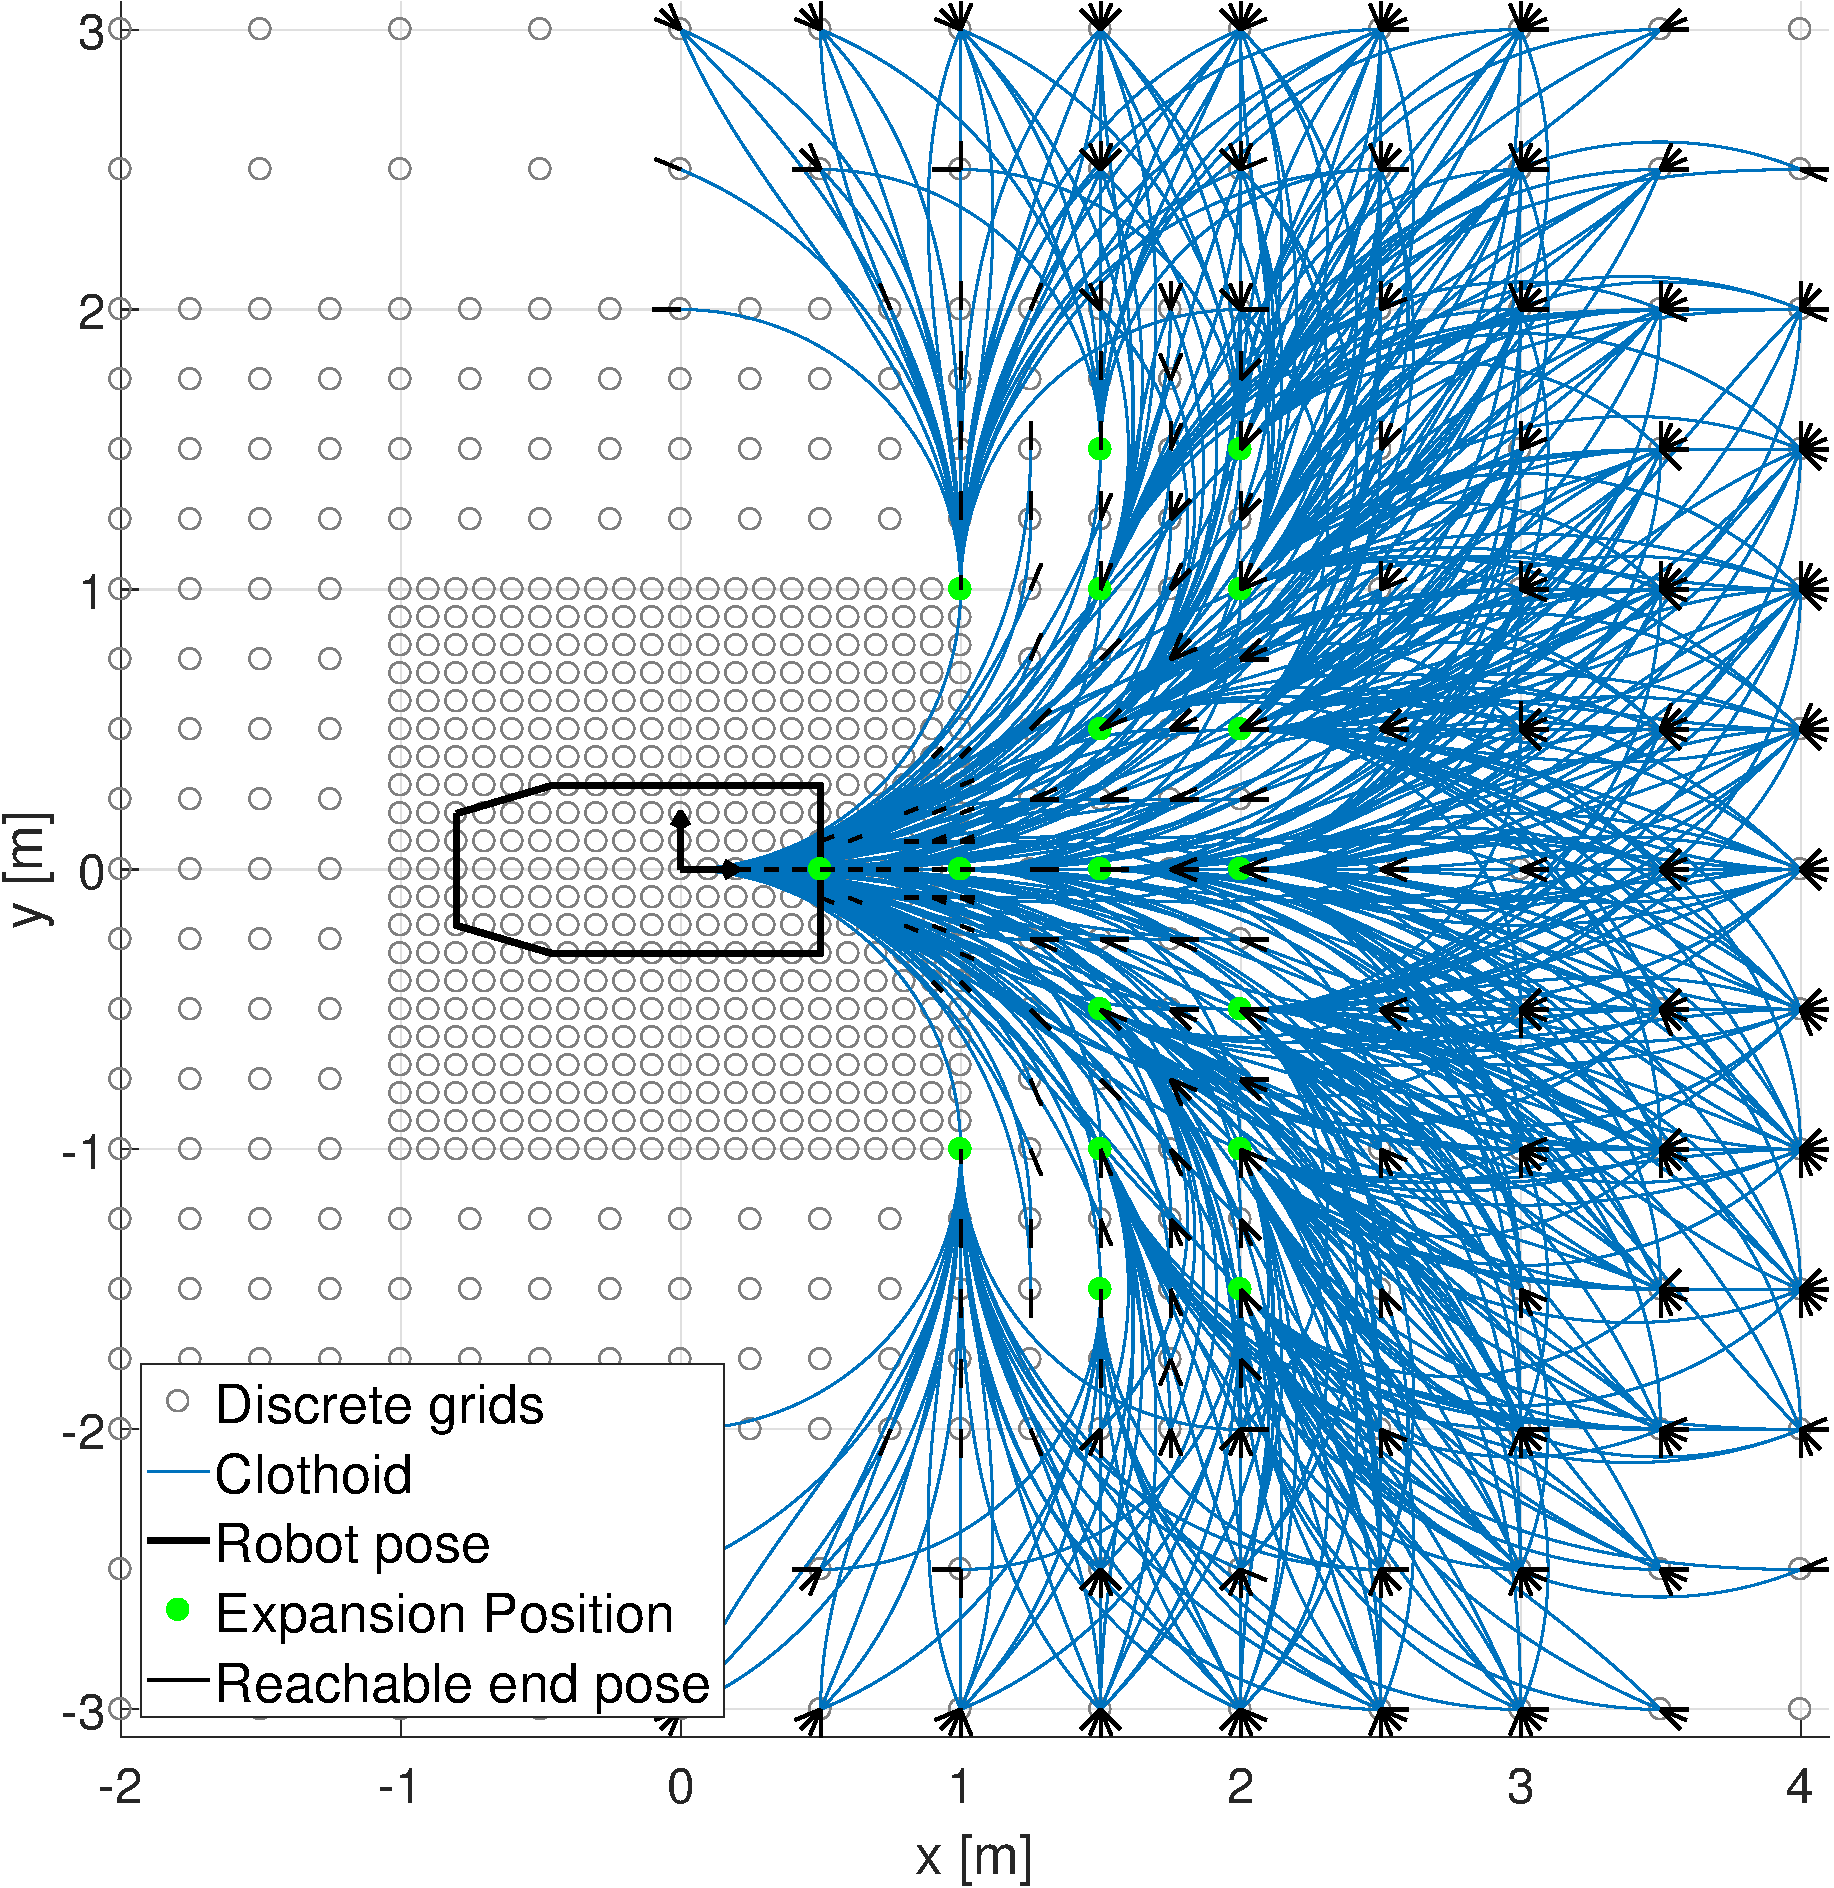
\includegraphics[width=\textwidth]{LSLClothoid.pdf}
	\doublecaption{A LSL based on clothoids}{is finally obtained after repeating the procedure shown in \cref{fig:MultiGirdWithEPROI} at every EP. This connects every feasible end pose close to the robot whilst moving forward with one or two clothoids. Backward movements and on-the-spot-turning are also implemented but are not illustrated in the present figure to maintain visibility. 
	\label{fig:LSLClothoid}}
\end{figure}

\newpage

\begin{table}[!htp]
%\vspace{0.25cm}
\centering
\doublecaption{Representation of the LSL data structure for a single path.}{This structure includes all necessary information to represent each path in the LSL and comprises precomputed data ($\bm{XY\Theta}, \bm{s},\bm{\kappa}$). These vectors contain the position and orientation, path length and curvature along each path, discretized in such a way that $\bm{s_{k+1}}-\bm{s_{k}} < res_{path}$. The $blockIdx$ entry represents the row index at which a certain path is blocked, meaning that if the row index is increased by one, the path will result in a collision with the environment. By default, this index is put to $rowlength(\bm{XY\Theta})+1$, meaning that the path should not be shortened. Finally, each path has a unique $ID$. \label{tab:LSLstruct}}
\begin{tabular}{|c|c|c|c|c|c|c|c|c|c|c|c|c|c|}
\hline
$\bm{p_0}$	&$ \bm{p_1}$	& $L_{tot}$	& $\kappa_0$		& $\kappa'$	& $\bm{XY\Theta}$	& $\bm{s}$ 	& $\bm{\kappa}$	& $blockIdx$ & $ID$	\\ \hline
1x3					& 1x3 					& 0.516		& 0.78						&-0.05				& 52×3						& 52×1						& 52×1		& 53				& 14		\\ \hline
\end{tabular}
\end{table}
%\vspace{0.25cm}
\begin{algorithm}[!bp]
\doublecaption{Overview of the LSL Algorithm}{computing the structure ($\mathcal{LSL}$) shown in \cref{tab:LSLstruct}. Each new entry (row) in this structure represents a feasible path ($\mathcal{P}$). Paths are added incrementally to the structure in line 9 and 19. The dot-operator (.) is used to access individual fields of each path of $\mathcal{LSL}$.
\label{alg:LSL}}
\begin{algorithmic}[1]
\Require{$userSettings$ to create matrix $\bm{P_{grid}}$ containing all discrete poses $\bm{p_{grid,k}}$.}
\Ensure{LSL Structure ($\mathcal{LSL}$) containing a set of feasible paths ($\mathcal{P}$).}
\LeftComment{calculate feasible paths at origin}
\State $\bm{p_0} \gets [0, 0, 0] $
\State $\bm{P_{grid}} \gets$ \Call{CreateMultiSizeGrid}{$userSettings$} 
\ForAll{$ \bm{p_{grid,i}} \in \bm{P_{grid}}$}
	\If{\Call{isInROI}{$\bm{p_{grid,i}},\bm{p_{0}} $}}
	\State $ \bm{p_1} \gets \bm{p_{grid,i}} $ 
	\State$[\bm{x},\bm{y},\bm{\theta},\bm{s},\bm{\kappa}] \gets $ \Call{getClothoidData}{$\bm{p_0},\bm{p_1}$}
		\If{$ \norm{\bm{\kappa}}_{\infty} \le \kappa_{max}$}
			\State $\mathcal{P} \gets [\bm{p_0},\bm{p_1},\bm{x},\bm{y},\bm{\theta},\bm{s},\bm{\kappa}]$
			\State $\mathcal{LSL} \gets $ \Call{addPathToLSLstruct}{$\mathcal{LSL,P}$}
		\EndIf
	\EndIf
\EndFor
\LeftComment{calculate feasible paths at Expansion Positions}
\ForAll{$ \mathcal{P} \in \mathcal{LSL}$ }
	\If{\Call{isExpansionPosition}{$\mathcal{P}.\bm{p_1}$}}
			\State $\bm{p_{0}} \gets \mathcal{P}.\bm{p_1} $ \Comment{end pose path $\mathcal{P}$ becomes start pose for next paths}
		\ForAll{$ \bm{p_{grid,i}} \in \bm{P_{grid}}$}
			\If{\Call{isInROI}{$\bm{p_{grid,i}},\bm{p_{0}} $}}
			\State $ \bm{p_1} \gets \bm{p_{grid,i}} $ 
			\State$[\bm{x},\bm{y},\bm{\theta},\bm{s},\bm{\kappa}] \gets $ \Call{getClothoidData}{$\bm{p_0},\bm{p_1}$}
				\If{$ \norm{\bm{\kappa}}_{\infty} \le \kappa_{max}$}
					\State $\mathcal{P} \gets [\bm{p_0},\bm{p_1},\bm{x},\bm{y},\bm{\theta},\bm{s},\bm{\kappa}]$
					\State $\mathcal{LSL} \gets $ \Call{addPathToLSLstruct}{$\mathcal{LSL,P}$}
				\EndIf
			\EndIf
		\EndFor
	\EndIf
\EndFor
\State $\mathcal{LSL} \gets $ \Call{CleanUpLSL}{$\mathcal{LSL}$} \Comment{Remove non-unique paths}
%\Function{ROI}{$\mathbf{p_{robot}}$}
%\State \Return $\mathbf{x,y,\theta,s,\kappa}$
%\EndFunction
\end{algorithmic}
\end{algorithm}

\newpage

\section{Lookup table for collision checking} \label{sec:LTCC}
Once the set of feasible trajectories used for the clothoidal LPT are defined, a lookup table is constructed offline to quickly evaluate online which paths are collision-free and to adjust their length if needed. Traditionally, this is done by the path-based approach, discussed in \cref{sec:PBLT}. A more efficient collision checking method was developed in \cite{DemeesterEtAl2012}, called the obstacle-based approach shown in \cref{sec:OBLT}. But first, the calculation of the OG for each path is presented in \cref{sec:OGC}.

\subsection{Calculating the occupancy grid for each path} \label{sec:OGC}
%TODO
% NOT CLEAR to ensure that a cell of the OG does not travel more than one cell between two discrete poses on the path (concrete values given in \cref{tab:LSLParVal}).
The first step of the creation of the (path- or obstacle-based) lookup table is to calculate the OG of each path. This is the space that the wheelchair will occupy when moving along this particular trajectory. The LSL structure defined in \cref{tab:LSLstruct} contains all the information needed to reconstruct the calculated paths. The path index ($pathIdx$) is the row index of $\bm{XY\Theta}$. This matrix contains all the discrete poses the sAMR will adopt while following the path between the start pose $\bm{p_0}$ and the end pose $ \bm{p_1}$. The same row index can be used to access other information, such as current path length ($\bm{s}$) or path curvature ($\bm{\kappa}$). The resolution for every curve is fixed at $\bm{s}(k) - \bm{s}(k-1) = res_{path} < res_{OG}/2$ to ensure that a cell of the OG does not travel more than one cell between two discrete poses on the path (concrete values given in \cref{tab:LSLParVal}).

The OG of the robot at the origin is shown in \cref{fig:OGRobotStart}. In order to improve performance, two OGs are used. One full OG is applied at every start of the path and a shell OG is used for the following steps to obtain a faster computation of the path OG. Since one occupied grid will not move more than once cell per step, there is no loss of information when using the shell OG representation for the wheelchair.

As the sAMR moves along the path, grid cells that were not visited during the previous steps are stored, along with the current path index and path ID. This procedure is shown in \cref{fig:OGRobotPath}. The reason for storing this path index is to be able to adjust the path length in the presence of obstacles. If only the visited cells were stored, path length adjustments would be impossible and the whole path would be judged as blocked.

Although row indexes correspond to geometrical information (the position along the path), these data could be used to forecast positioning and obstacle avoidance assuming that the robot drives at a constant velocity. 

The way that this particular information is stored will play a crucial role in the time performances of the online collision checking method. This will be explained in the following sections.

\newpage

\begin{figure}[!htbp]
\centering
	\begin{minipage}[b]{.45\linewidth}
		\centering
		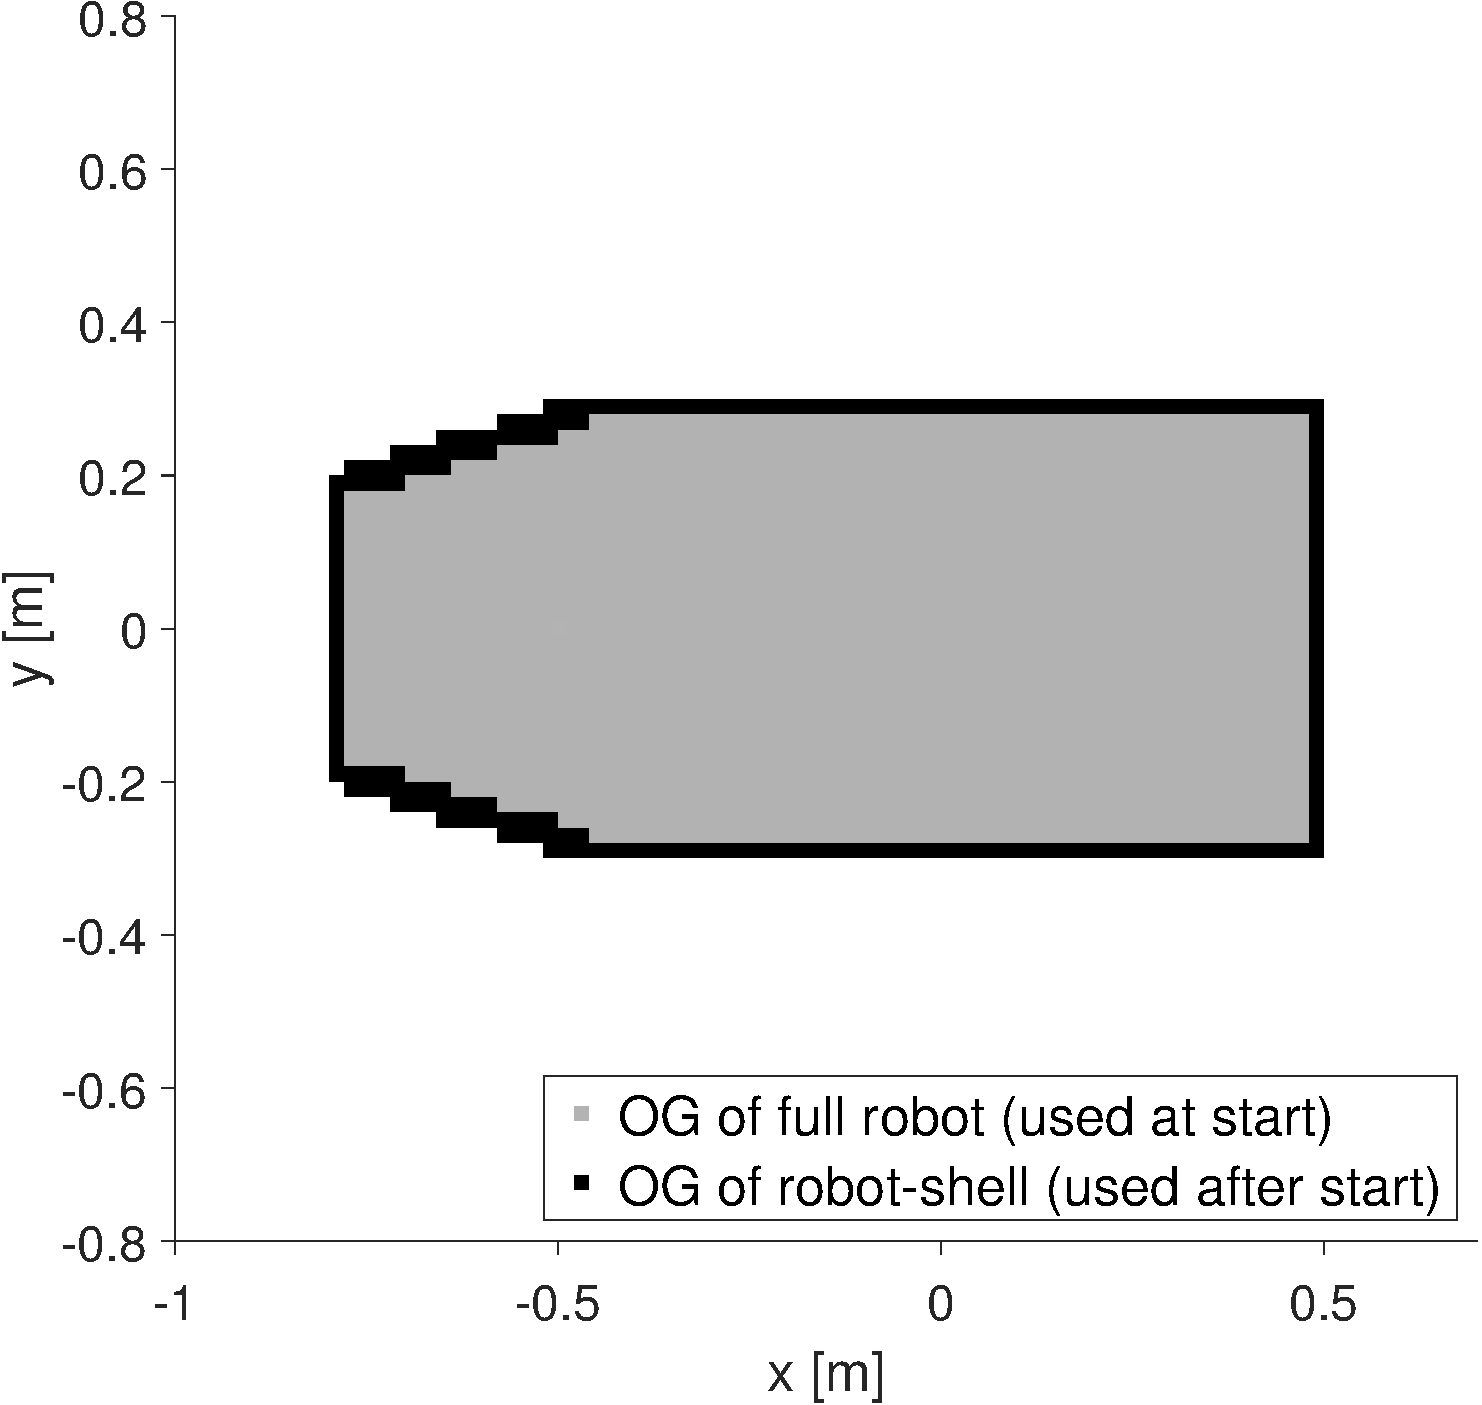
\includegraphics[width=\textwidth]{OGRobotStart.pdf}
	\end{minipage}
	\hfill%
	\centering
	\begin{minipage}[b]{.45\linewidth}
		\centering
		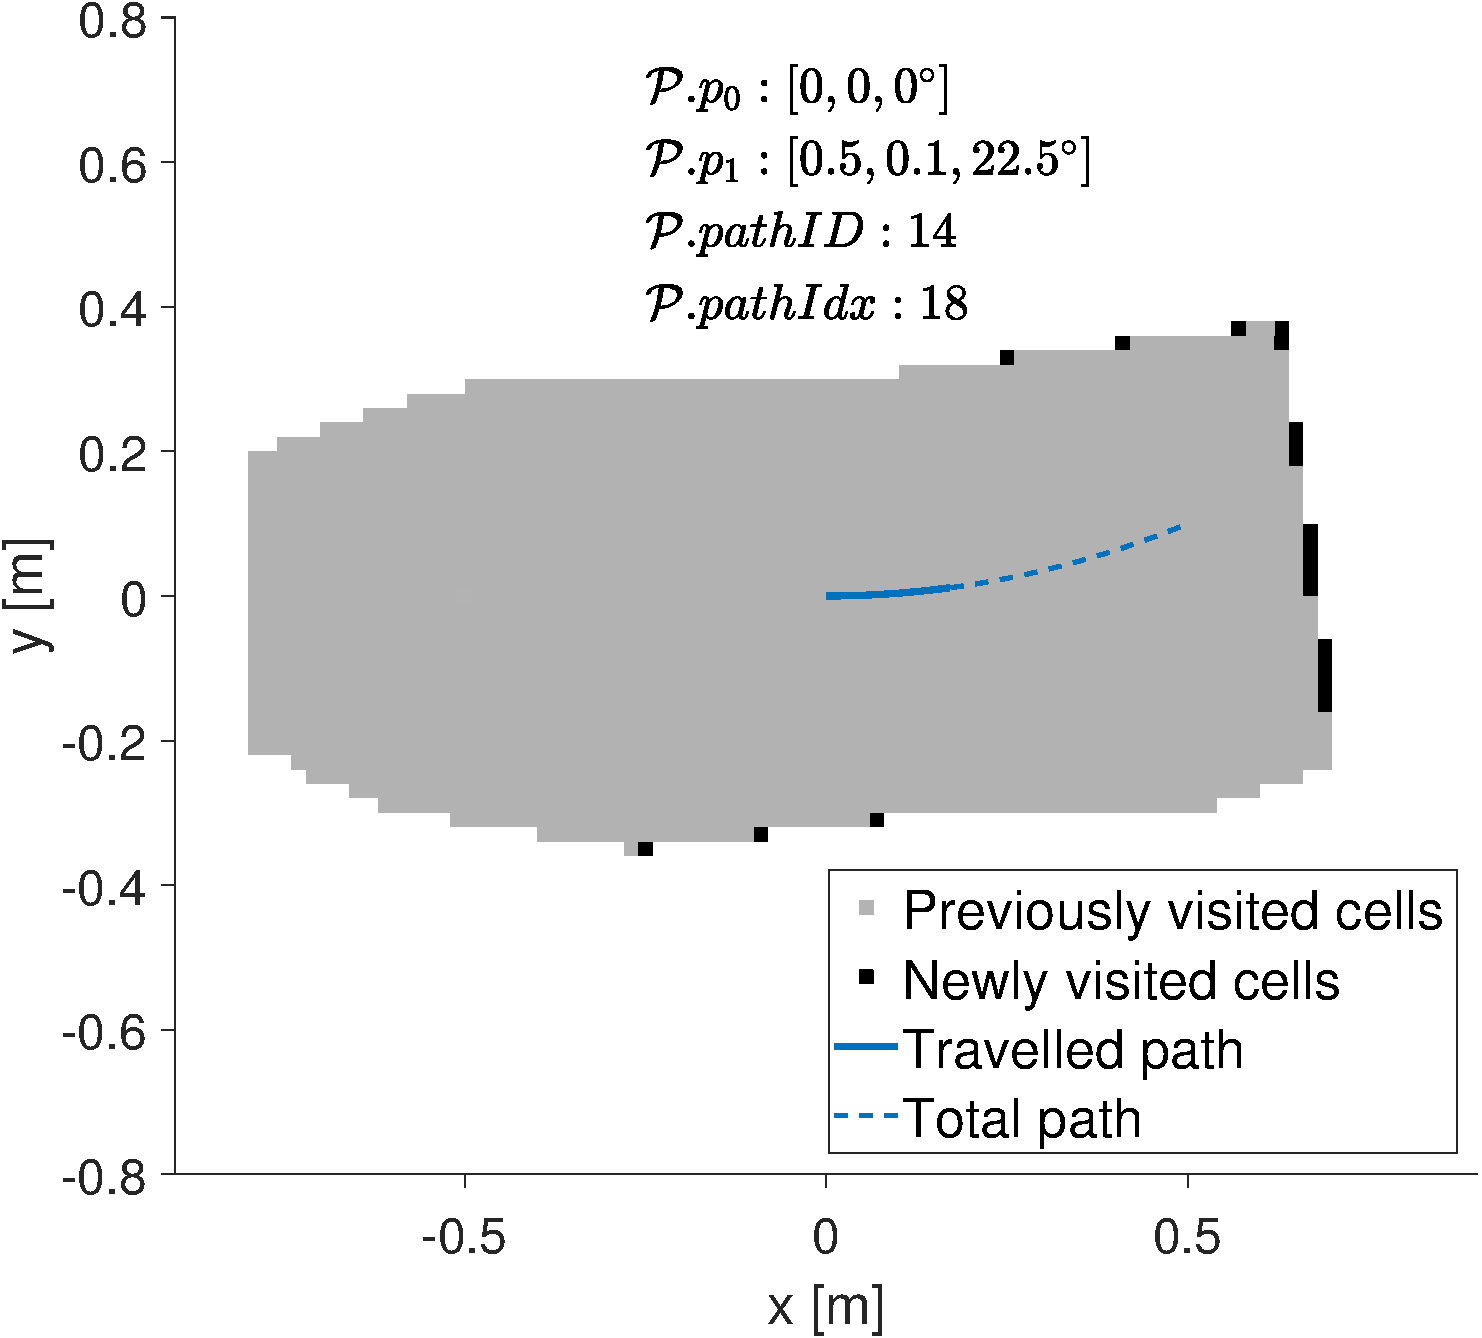
\includegraphics[width=\textwidth]{OGRobotPath.pdf}
	\end{minipage}\\[-7pt]
	\begin{minipage}[t]{.45\linewidth}
		\doublecaption{Two OGs are used to represent the wheelchair's footprint.}{The OG of the full robot is used just once, at the start of the path. The robot-shell OG is used for the remainder of the path. This approach significantly reduces calculation time. Note that the OG of the full robot also consists of the shell robot, although not shown in the graph. \label{fig:OGRobotStart}}
	\end{minipage}
	\hfill
	\begin{minipage}[t]{.45\linewidth}
		\doublecaption{The Path OG is created by moving the wheelchair along the path.}{Each time a grid cell is visited for the first time, it is stored along with the path-ID and path-index. This path-index represents the position along the path. The distance between 2 path indices is at most equal to $res_{path}< res_{grid}/2$ to ensure that each cell in the OG travels at most one cell in the OG of the path. \label{fig:OGRobotPath}}
	\end{minipage}
\end{figure}
\vspace{-1.5cm}

\subsection{Path-based lookup table} \label{sec:PBLT}
The information calculated in the previous section should now be stored adequately to form a lookup table. Traditionally, all this information would be stored along with the path information, resulting in just an additional entry in the LSL structure shown in \cref{tab:LSLstruct} in the form of matrix $\bm{X_{occ}Y_{occ}pathIdx}$ for each path.

To evaluate if a path is occupied, each path is checked individually. If there is an overlap between the path OG and the grid map containing the perceived obstacles from the environment, the path length is adapted. To increase speed performance, the path-based lookup table should be sorted by ascending path index, in order to break the loop once the first obstacle on the path is met. This procedure is also displayed in \cref{alg:PBLT}. It is important to note that following this procedure for every path would result in checking several times the same occupied grid from the set of paths. This is in particular the case at the start of each path, since all trajectories share a common origin.

This has motivated the construction of a lookup table build in such a way that occupied cells from the paths are checked only once. This will be presented in the next section. A first result of the path length adjustment can be found in \cref{fig:LPT_LT}. The result will be the same regardless of the method used (path- or obstacle-based).

\begin{algorithm}
\doublecaption{Path-based lookup table}{(online phase)(adapted from \cite{DemeesterEtAl2012})\label{alg:PBLT}}
\begin{algorithmic}[1]
%\Statex
%\Require{$LSL$: }
%\Ensure{Output}
\Statex
\ForAll{$ \mathcal{P} \in \mathcal{LSL}$ }
\State $\mathcal{P}.blockIdx \gets \Call{rowLength}{\mathcal{P}.\bm{XY\Theta}}+1$ \Comment{initialize path $\mathcal{P}$ as free}
\ForAll{$ \mathcal{C} \in \Call{getCellsOccupiedByPath}{\mathcal{P}}$}
\If{$\Call{gridMapEnviroment}{\mathcal{C}}==occupied$}
\State $\mathcal{P}.blockIdx \gets $ \Call{lookupTableBlockIdx}{$\mathcal{P},\mathcal{C}$}
\State \textbf{break} \Comment{proceed with next path}
\EndIf
\EndFor
\EndFor
\end{algorithmic}
\end{algorithm}

\begin{algorithm}
\doublecaption{Obstacle-based lookup table}{(online phase)(adapted from \cite{DemeesterEtAl2012})\label{alg:OBLT}}
\begin{algorithmic}[1]
%\Statex
%\Require{$LSL$: }
%\Ensure{Output}
\Statex
\ForAll{$ \mathcal{P} \in \mathcal{LSL}$ }
\State $\mathcal{P}.blockIdx \gets \Call{rowLength}{\mathcal{P}.\bm{XY\Theta}}+1$ \Comment{initialize path $\mathcal{P}$ as free}
\EndFor
\ForAll{$ \mathcal{C} \in \Call{getCellsOccupiedByLSL}{\mathcal{LSL}}$}
\If{$\Call{gridMapEnviroment}{\mathcal{C}}==occupied$}
\ForAll{$ \mathcal{P} \in \Call{lookupTablePathsInCell}{\mathcal{C}} $}
\If{$\mathcal{P}.blockIdx >$ \Call{lookupTableBlockIdx}{$\mathcal{C,P}$}}
\State $\mathcal{P}.blockIdx \gets $ \Call{lookupTableBlockIdx}{$\mathcal{C,P}$}
\EndIf
\EndFor
\EndIf
\EndFor
\end{algorithmic}
\end{algorithm}

\subsection{Obstacle-Based Lookup Table} \label{sec:OBLT}
From the previous section, it is clear that the construction of the lookup table itself can be optimized, to ensure that each cell is only checked once, while still containing all the information needed to adapt a path length to avoid collision \cite{DemeesterEtAl2012}.

The lookup table is therefore constructed based on the occupied cells by the wheelchair when taking the paths from the LPT. Each cell in this table represents a location that is occupied by the OG of one or more paths from the LSL. The $pathID$ and $pathIdx$ of each trajectory occupying this cell is also provided in that cell. Once this table is build, the occupied cells in the grid map representing the environment have to be matched with the cells in the lookup table. If there is a match, each path length is updated by the provided information of that cell ($pathID$ and $pathIdx$). Note that this only takes place if this reduces the path length. This procedure is also displayed in \cref{alg:OBLT}. 

An example of the path length adjustment is illustrated in \cref{fig:LPT_LT}. The obtained result is regardless of the chosen method, but the obstacle-based lookup table is more efficient compared to the path-based obstacle table due to its improved construction. A single entry of the obstacle-based lookup table data structure can be found in \cref{tab:OBLTstruct}.

\begin{table}[!htp]
\centering
\doublecaption{Representation of a single cell of the obstacle-based lookup table data structure.}{The entries $x$ and $y$ represent the location of the occupied grid cell by the robot (up to a resolution $res_{grid}=2cm$) and contain all the paths (represented by $pathID$) occupying this particular cell along with the corresponding path length when this cell is occupied for the first time by this particular path (represented by $pathIdx$, the row index of $\bm{XY\Theta}$). This cell is the occupied cell shown in \cref{fig:LPT_LT} at the top right corner. \label{tab:OBLTstruct}}
\begin{tabular}{|c|c|c|c|}
\hline
$x$			&		$y$		& $pathID$ 						& $pathIdx$				\\ \hline
$3.90m$	& $2.96m$ & $[763,764,779]$			& $[202,192,226]$	\\ \hline
\end{tabular}
\end{table}

\begin{figure}[!htbp]
\centering
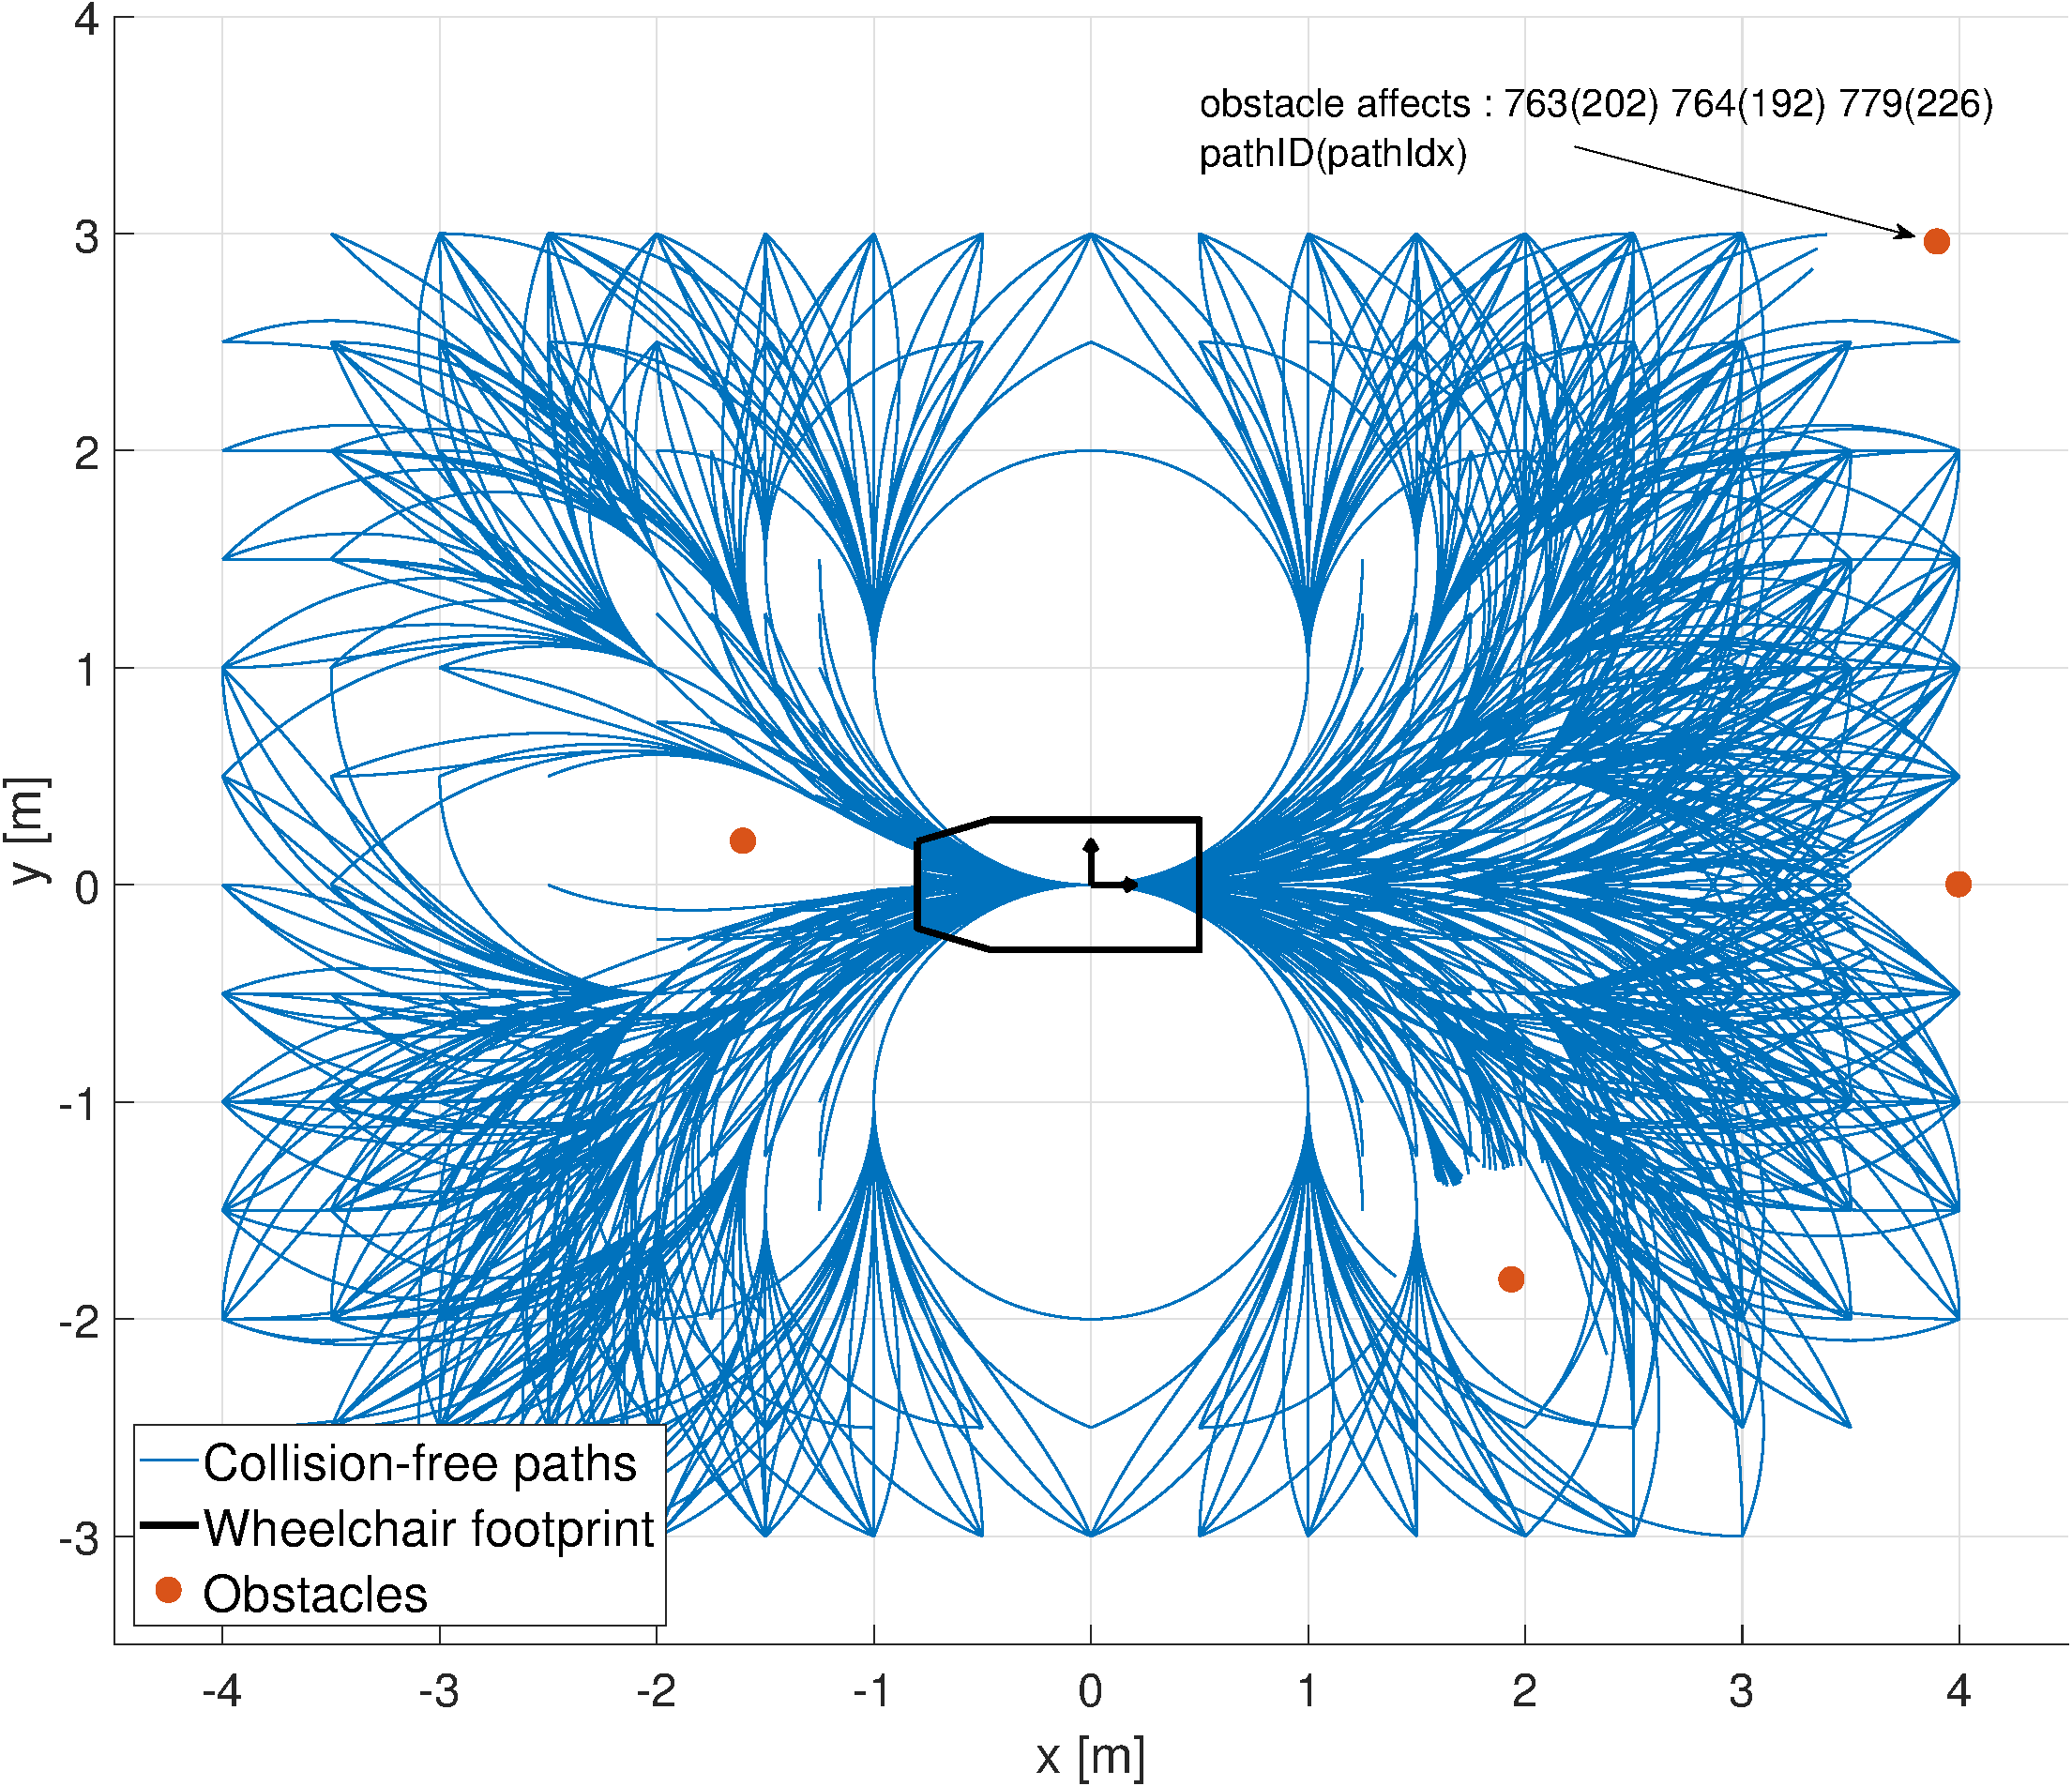
\includegraphics[width=0.95\textwidth]{LPT_LT.pdf}
\doublecaption{Example of the path length adjustment by the LPPA with 3 obstacles points.}{Each obstacle is exactly one grid cell (although inflated on the figure for readability). The influence on each path of the top right obstacle is shown.
\label{fig:LPT_LT}}
\end{figure}

\newpage

\section{Extention for Dynamic Motion Planning} \label{sec:DynPlan}
In the previous sections of this chapter, the focus of the developed LPPA has been on the geometry of the curve and its path length adaptation for static obstacles. This still leaves an important gap in terms of real-life operability of the LPPA as it does not prevent collisions with dynamic obstacles crossing the path taken by the sAMR. Such a situation is shown in \cref{fig:DVP_Start}. The solution put forward to avoid such collisions relies on the strength of the LPT (i) to perform path adjustments for static obstacles and (ii) to calculate an optimal speed profile ($v(t)$) to achieve a collision-free motion avoiding dynamic obstacles. This optimal speed profile is calculated by applying the methods described in \Cref{sec:OMGreview}, but for a fixed path, therefore reducing the computational cost for the calculation of the COP. This method assumes a given motion model for each obstacle and an OG representing their shape. There is however no restriction to the path or the shape (convex or concave) of the obstacles.

\Cref{sec:STspace} explains the creation of the distance-time collision space ($s,t-$space) where $s$ is the distance along a fixed path. This collision space will be used for a COP described in \cref{sec:OSPCOP}, using a dynamic model of the wheelchair along with time-varying separating hyperplanes (shown \cref{fig:SeparatingHyperPlane}) to provide collision-free motion by finding an optimal speed profile to reach the end of a given path.

\begin{figure}[!htbp]
\centering
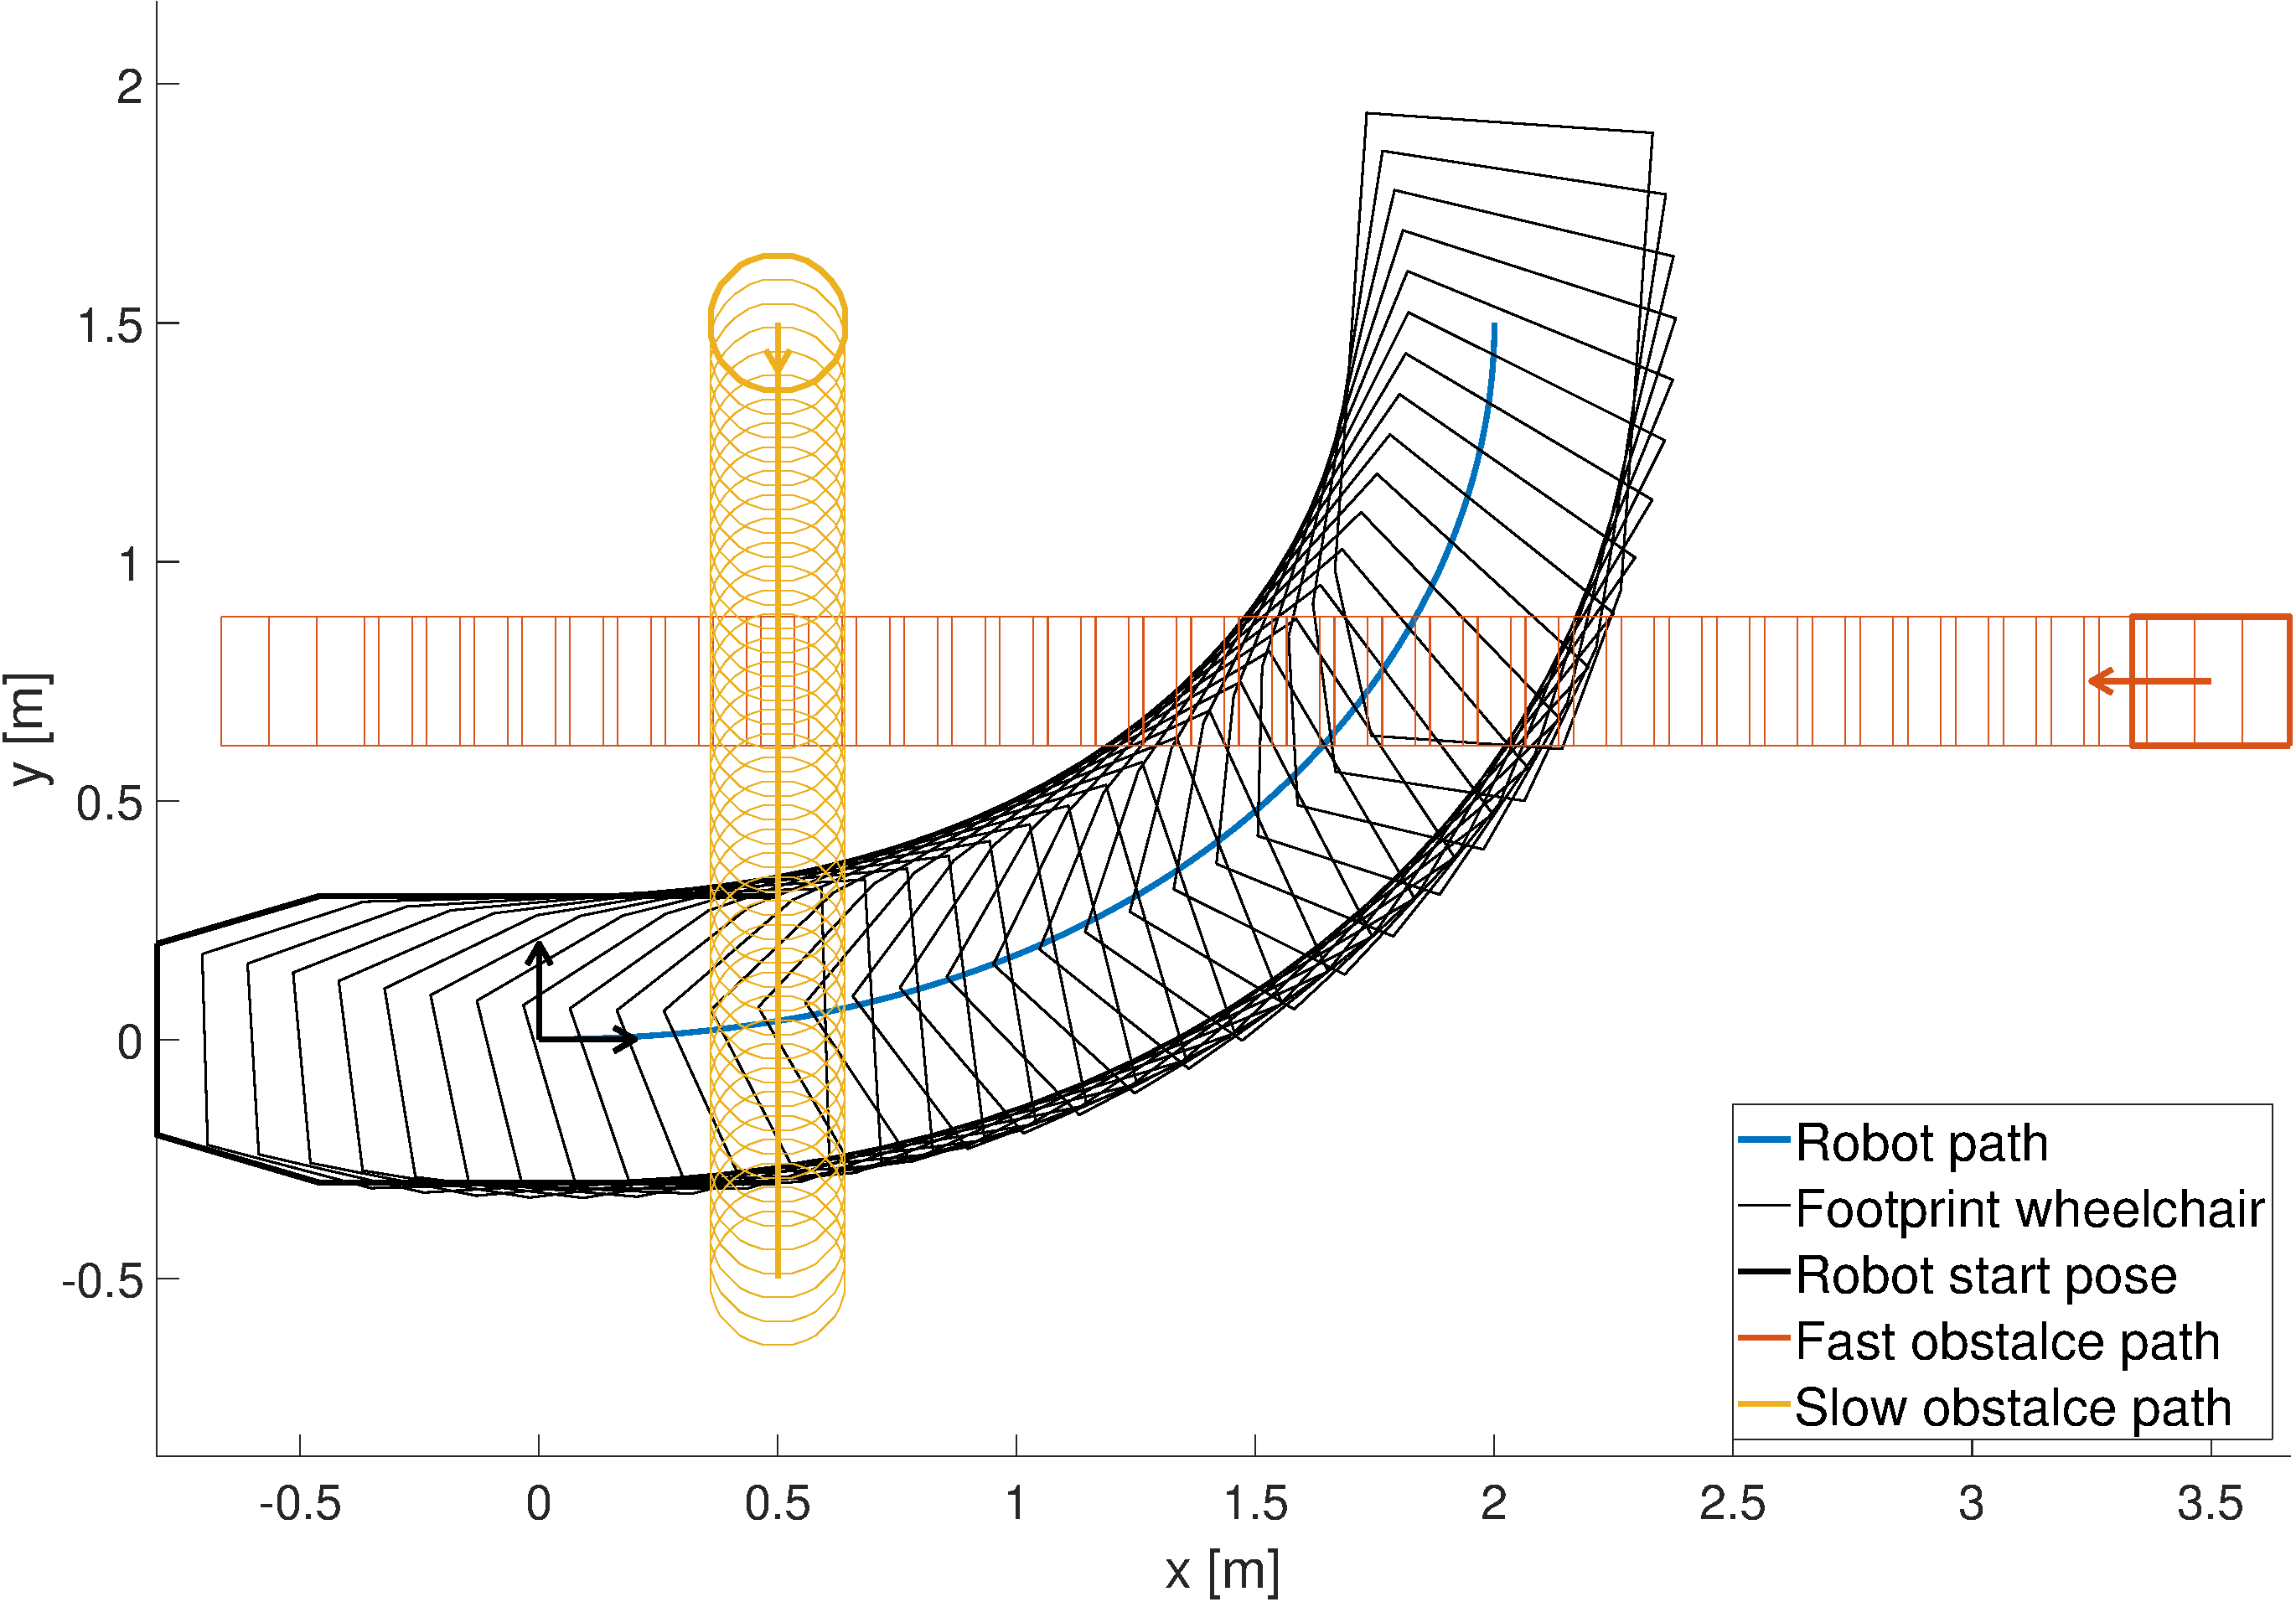
\includegraphics[width=0.9\textwidth]{DVP_Start.pdf}
\doublecaption{Dynamic obstacles potentially causing a collision with the sAMR.}{For clarity, only the shell of the dynamic obstacles’ OG are shown.
\label{fig:DVP_Start}}
\end{figure}

\newpage

\subsection{Distance-time collision space} \label{sec:STspace}
The $s,t-$space can be seen as a grid, within which all collisions between the robot positioned at a certain distance along the fixed path and the time-varying position of the moving obstacle are calculated. The following procedure is followed to perform this calculation:
\begin{enumerate}
\item The full OG of the robot along the fixed path is used, to determine the first and last impact time of the moving obstacle. This will narrow the search space along the $t$-axis (\cref{fig:DVP_FirstLastImpact}, left).
\item The full OG of the moving obstacle is determined by integrating its velocity. The first and last position on the fixed robot-path colliding with the moving obstacle is calculated. This will narrow the search space along the $s$-axis (\cref{fig:DVP_FirstLastImpact}, right).
\item In the restricted space determined by ($[t_{first},s_{first}]-[t_{last},s_{last}]$), all discrete $s,t$ collision states are calculated, determined by the path resolution ($\Delta s$) and the time resolution ($\Delta t$). An example for a fixed time for the obstacle is shown in \cref{fig:DVP_TSocc} (left). Repeating this for every time instance results in the ($s,t-$space) diagram, indicating all the possible collision states shown in \cref{fig:DVP_TSocc} (right)
\item Further optimization can be performed on the obtained collision states. As time-varying separating hyperplanes will be used in the COP, it will be more efficient to only keep a convex shape of the obtained collision states. This convex shape can be further simplified when applying the following (logical) constraints: (i) implying that the sAMR can't move backwards and (ii) time always moves forward (to the right) results in a nearly rectangular shape determined by ($[t_{first},s_{first}]-[t_{last},s_{last}]$). The outcome is not always rectangular, as can be seen in a ($s,t-$space) for another obstacle in \cref{fig:DVP_Solution}.
\end{enumerate}

\begin{figure}[!htbp]
\centering
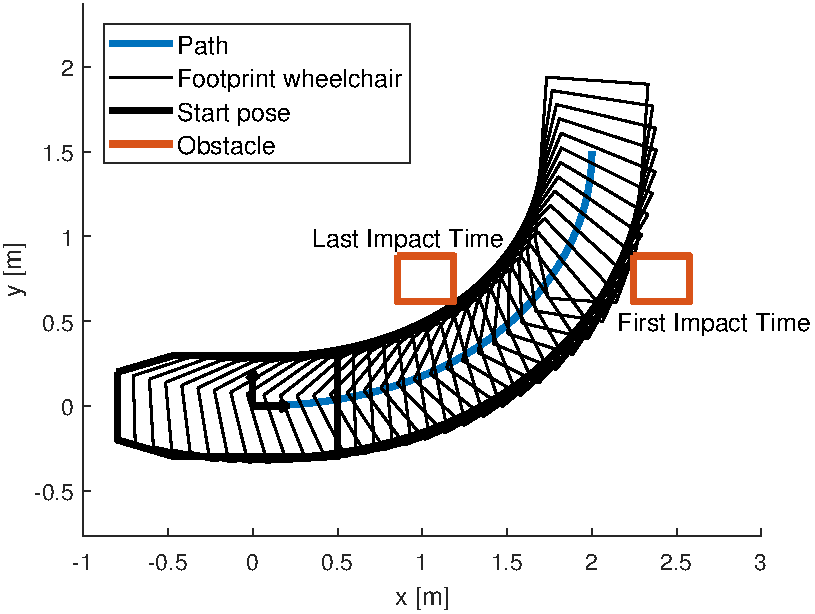
\includegraphics[width=0.49\textwidth]{DVP_FirstLastImpactTime.pdf}
\hfill
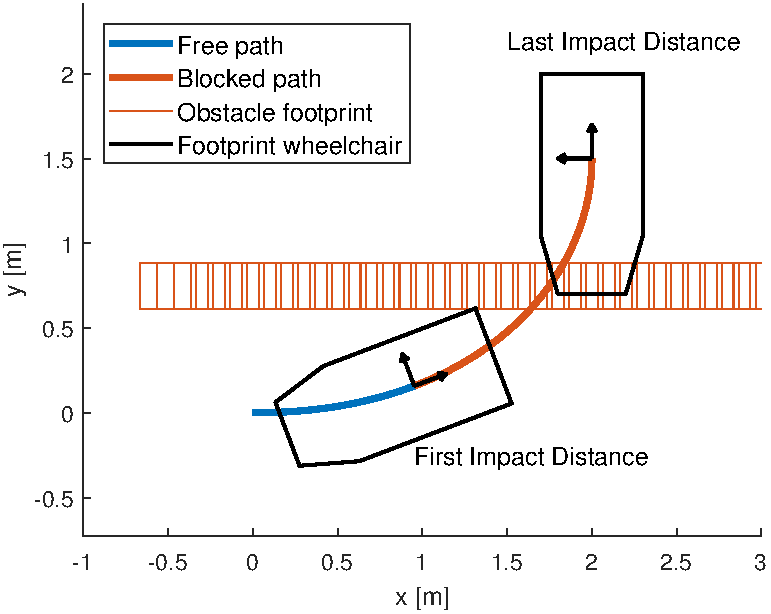
\includegraphics[width=0.49\textwidth]{DVP_FirstLastImpactDistance.pdf}
\doublecaption{First and last impact time and distance}{are calculated to reduce the computational time of the individual collision states in the  $s,t-$space
\label{fig:DVP_FirstLastImpact}}
\end{figure}

\begin{figure}[!htbp]
\centering
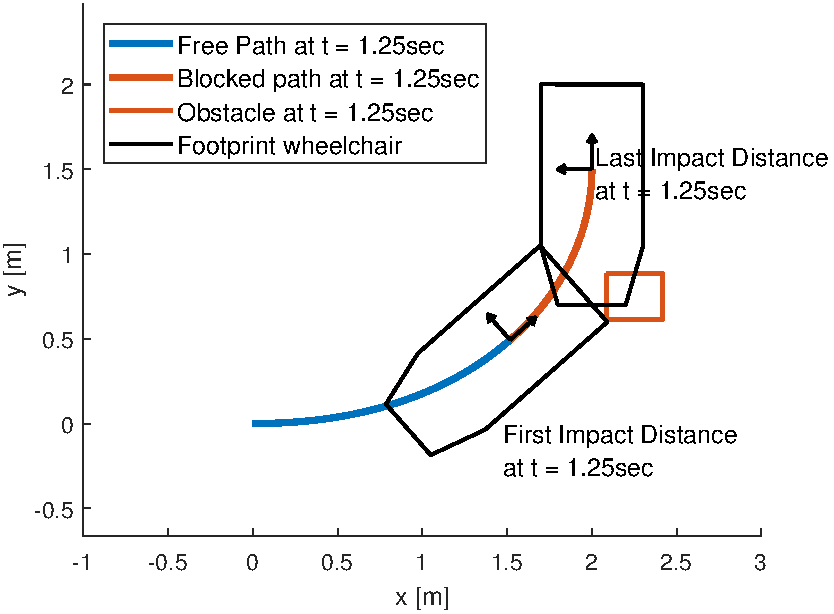
\includegraphics[width=0.49\textwidth]{DVP_FirstLastImpactDistance_FixedTime.pdf}
\hfill
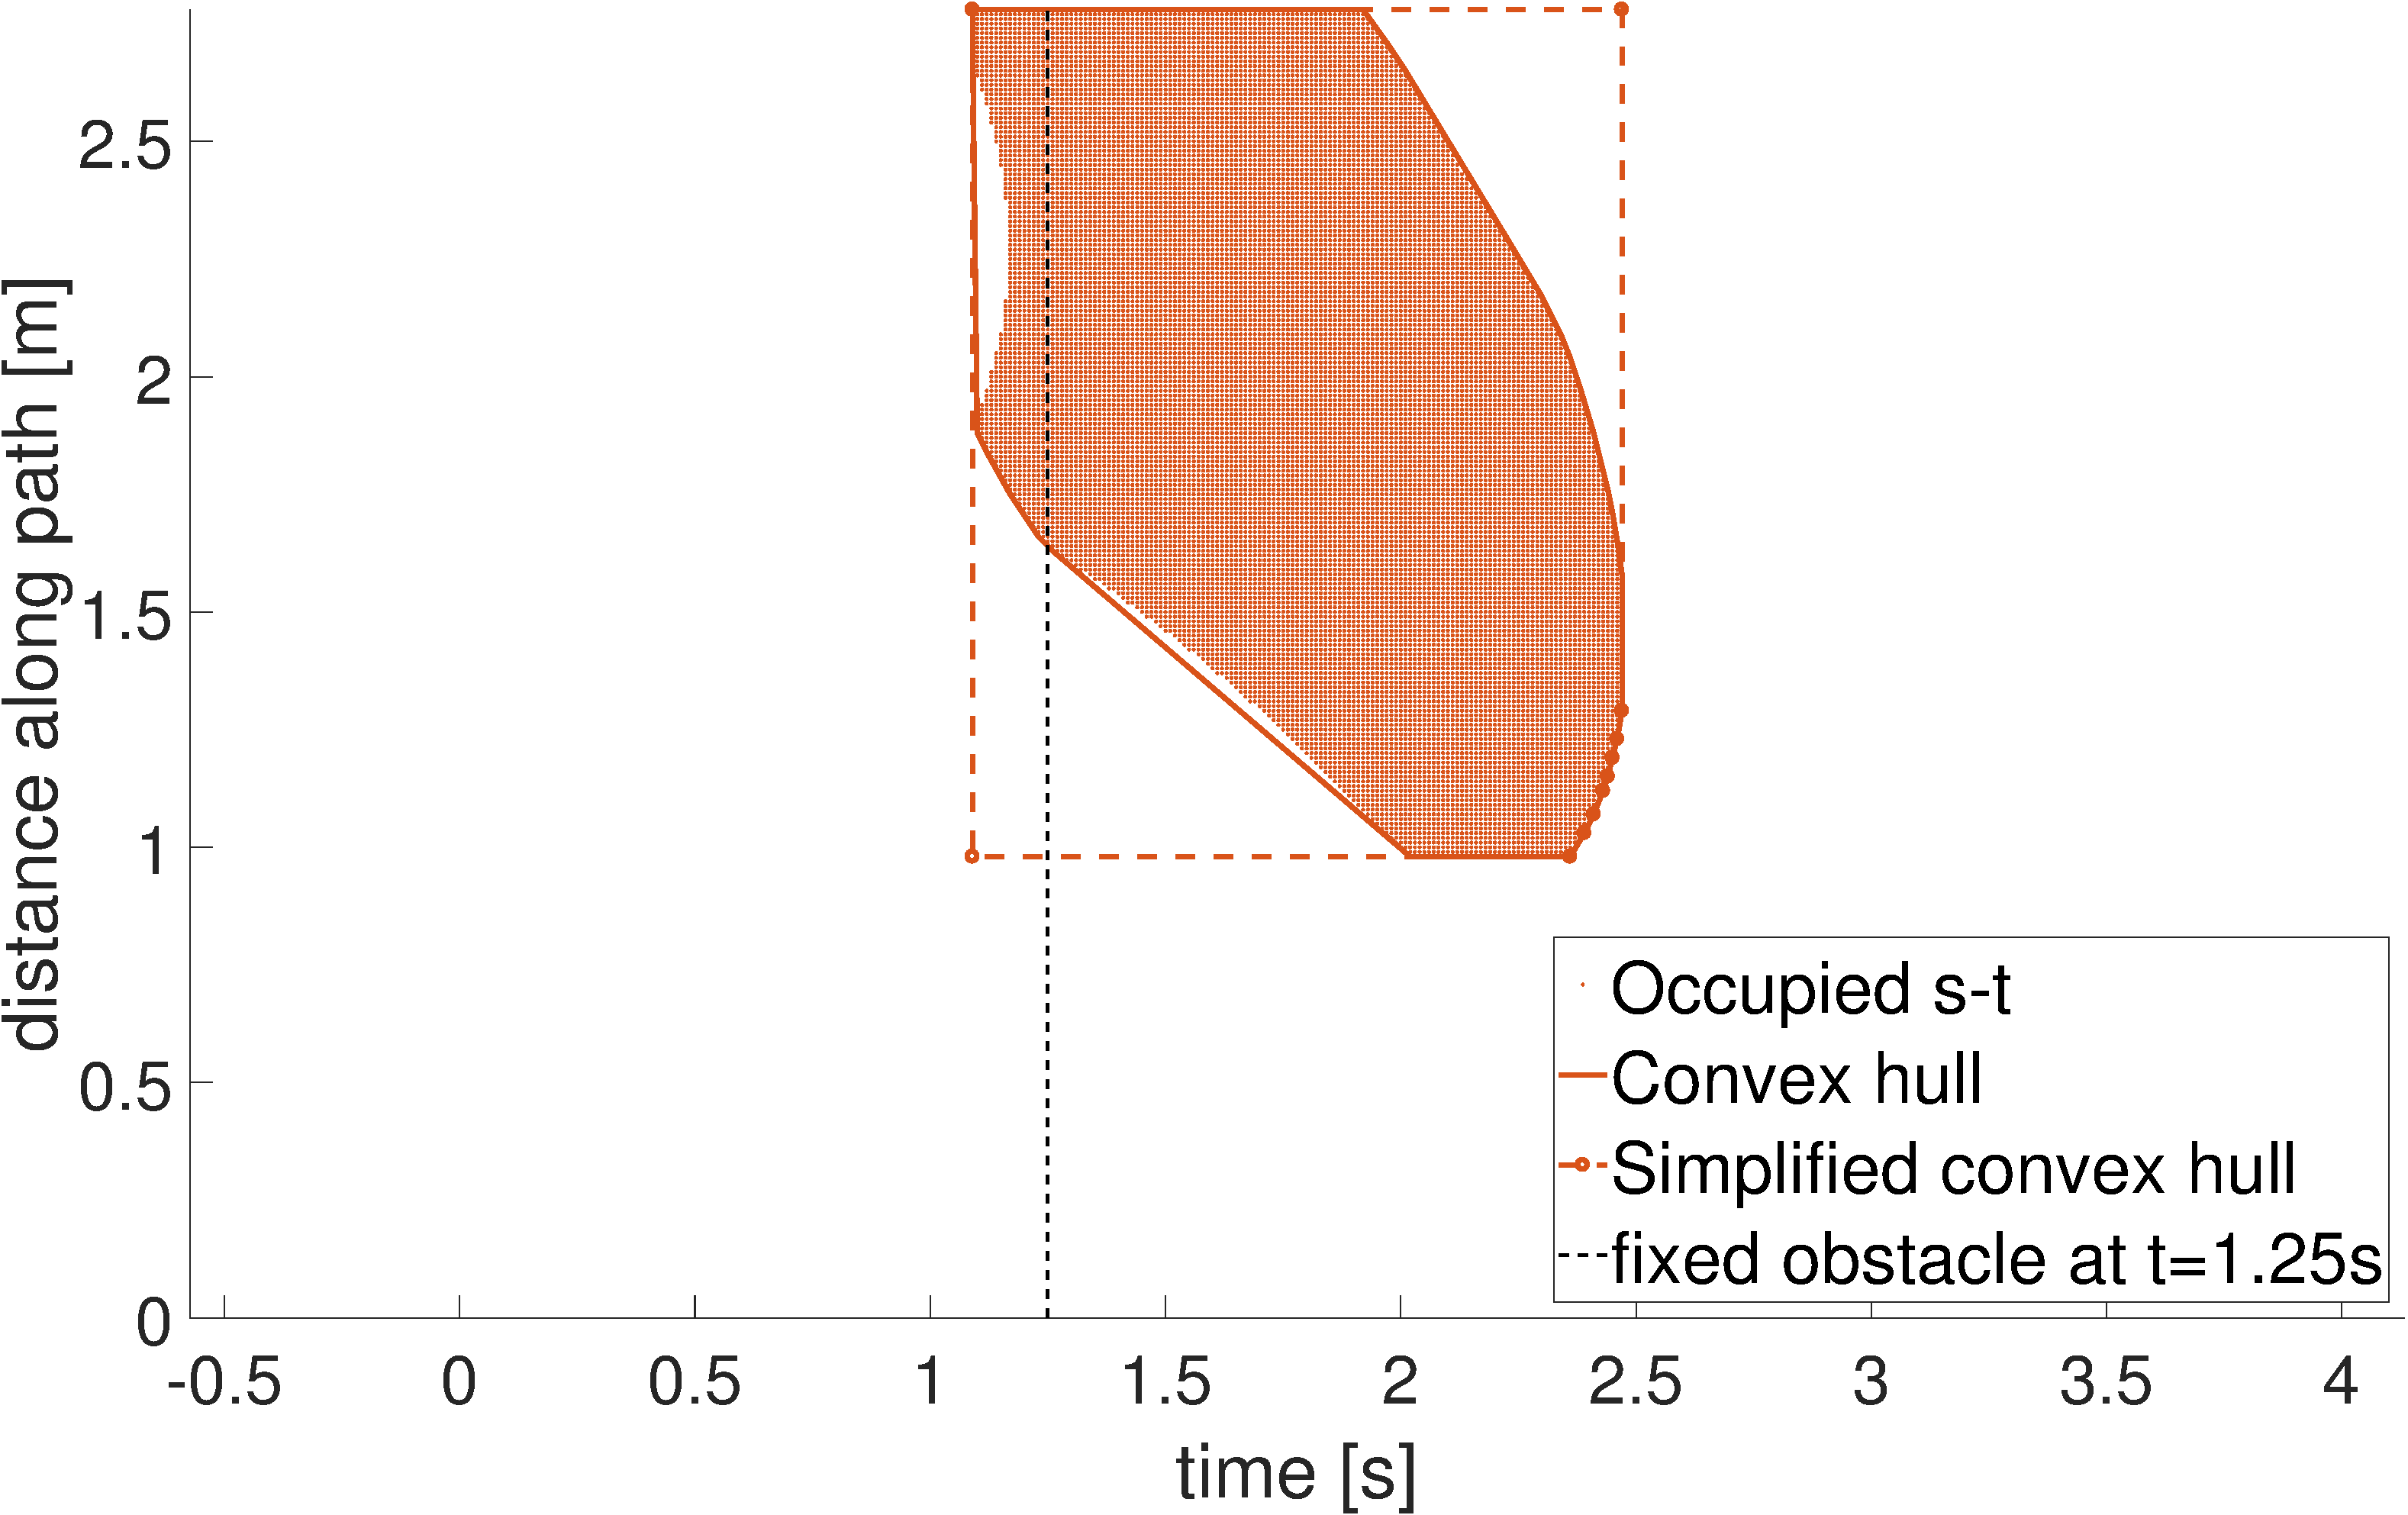
\includegraphics[width=0.49\textwidth]{DVP_TSocc_Diagram_Convex.pdf}
\doublecaption{(right) The distance-time collision space is obtained by calculating the discrete distance along the robot-path resulting in a collision at a certain time with the moving obstacle.}{The slashed vertical line at $t=1.25s$ corresponds to the situation shown on the left, where distances along the robot-path are marked in red for the position of the obstacle at $t=1.25s$.
\label{fig:DVP_TSocc}}
\end{figure}

\newpage

\subsection{Optimal speed profile calculation} \label{sec:OSPCOP}
A COP can be formulated to find an optimal speed profile given a distance-time collision space compliant with kinematic and dynamic constraints of the sAMR and an objective, which is to arrive within the minimum amount of time at the end of the path. This is shown in \cref{eq:DVP_COP}. This results in finding a path in the $s,t-$space, from position $[0,0]$ to $[\bm{s}(end), t_end]$ without colliding with the simplified convex hull of the collision states. This is shown in \Cref{fig:DVP_Solution}.

The COP is formulated based on the multiple-shooting approach, resulting in the discretization of the state along the path ($\bm{x}(t)=[s(t),v(t)]$) and force input $u(t)$ over a finite grid of $N$ samples. The model representing the wheelchair dynamics ($\bm{f}$) is then integrated with an integrator function ($\bm{I}$). For this conceptual solution, a simple mass-damper model was used. The time ($T$) needed to arrive at the end of the path ($\bm{s}(end)$) is kept as a decision variable, therefore an extra variable is defined, the variable time step $h=T/N$. Although not explicitly formulated in the COP, there is a one time-varying hyperplane for every moving obstacle, each requiring two parameters $\bm{a}(t)$ and $\bm{b}(t)$ (\cite{MercyEtAl2016}. $\bm{v}_{i}$ are the fixed vertices (positions) defining the simplified convex hull of the $s,t-$space. $r_{safe}$ is a safety factor, enforcing a minimum distance in the $s-t$ plane between obtained path and the simplified convex hull. Start conditions are enforced on both start distance and speed, but only an end distance is set as a constraint for the end state.

\begin{mini}[3]
{(\bm{x}_{1:N},u_{1:N},\bm{a}_{1:N},b_{1:N},T)}{T}
{\label{eq:DVP_COP}}{}
\addConstraint{\bm{x}_{k+1}}{=\bm{I}(\bm{f}(\bm{x}_{k},{u}_k,h), \, k=1\ldots N}
\addConstraint{{\bm{a}_{k}}^T\,\bm{v}_{i}-b_{k}}{\geqslant 0,  \, i=1: N_{vertices}} 
\addConstraint{{\bm{a}_{k}}^T\,\bm{x}_{k}-b_{k}}{\leqslant - r_{safe}} 
\addConstraint{\bm{x}_1}{= [0,v_{start}]} 
\addConstraint{\bm{x}_{N,1}}{= \bm{s}(end)} 
\addConstraint{ 0 \leqslant}{\ \bm{x}_ {k,2} \leqslant v_{max}} 
\addConstraint{u_{min} \leqslant}{\ u_k \leqslant u_{max}} 
\addConstraint{T\geqslant}{0} 
\addConstraint{\norm{\bm{a}_{k}}\leqslant}{1}
\end{mini}

%\vspace{2em}
The shape of the collision space will be approximately the same for two similar paths, therefore speeding up the calculation process by using a solution that has been found previously as initial start value for the next path. Increased computational speed can also be achieved by using a grid planner instead of a formal COP formulation. Planners designed with a fast re-planning capability (D* or Incremental Phi*) would greatly benefit from the similarity of the occupied $s,t-$space.

\begin{figure}[!htbp]
\centering
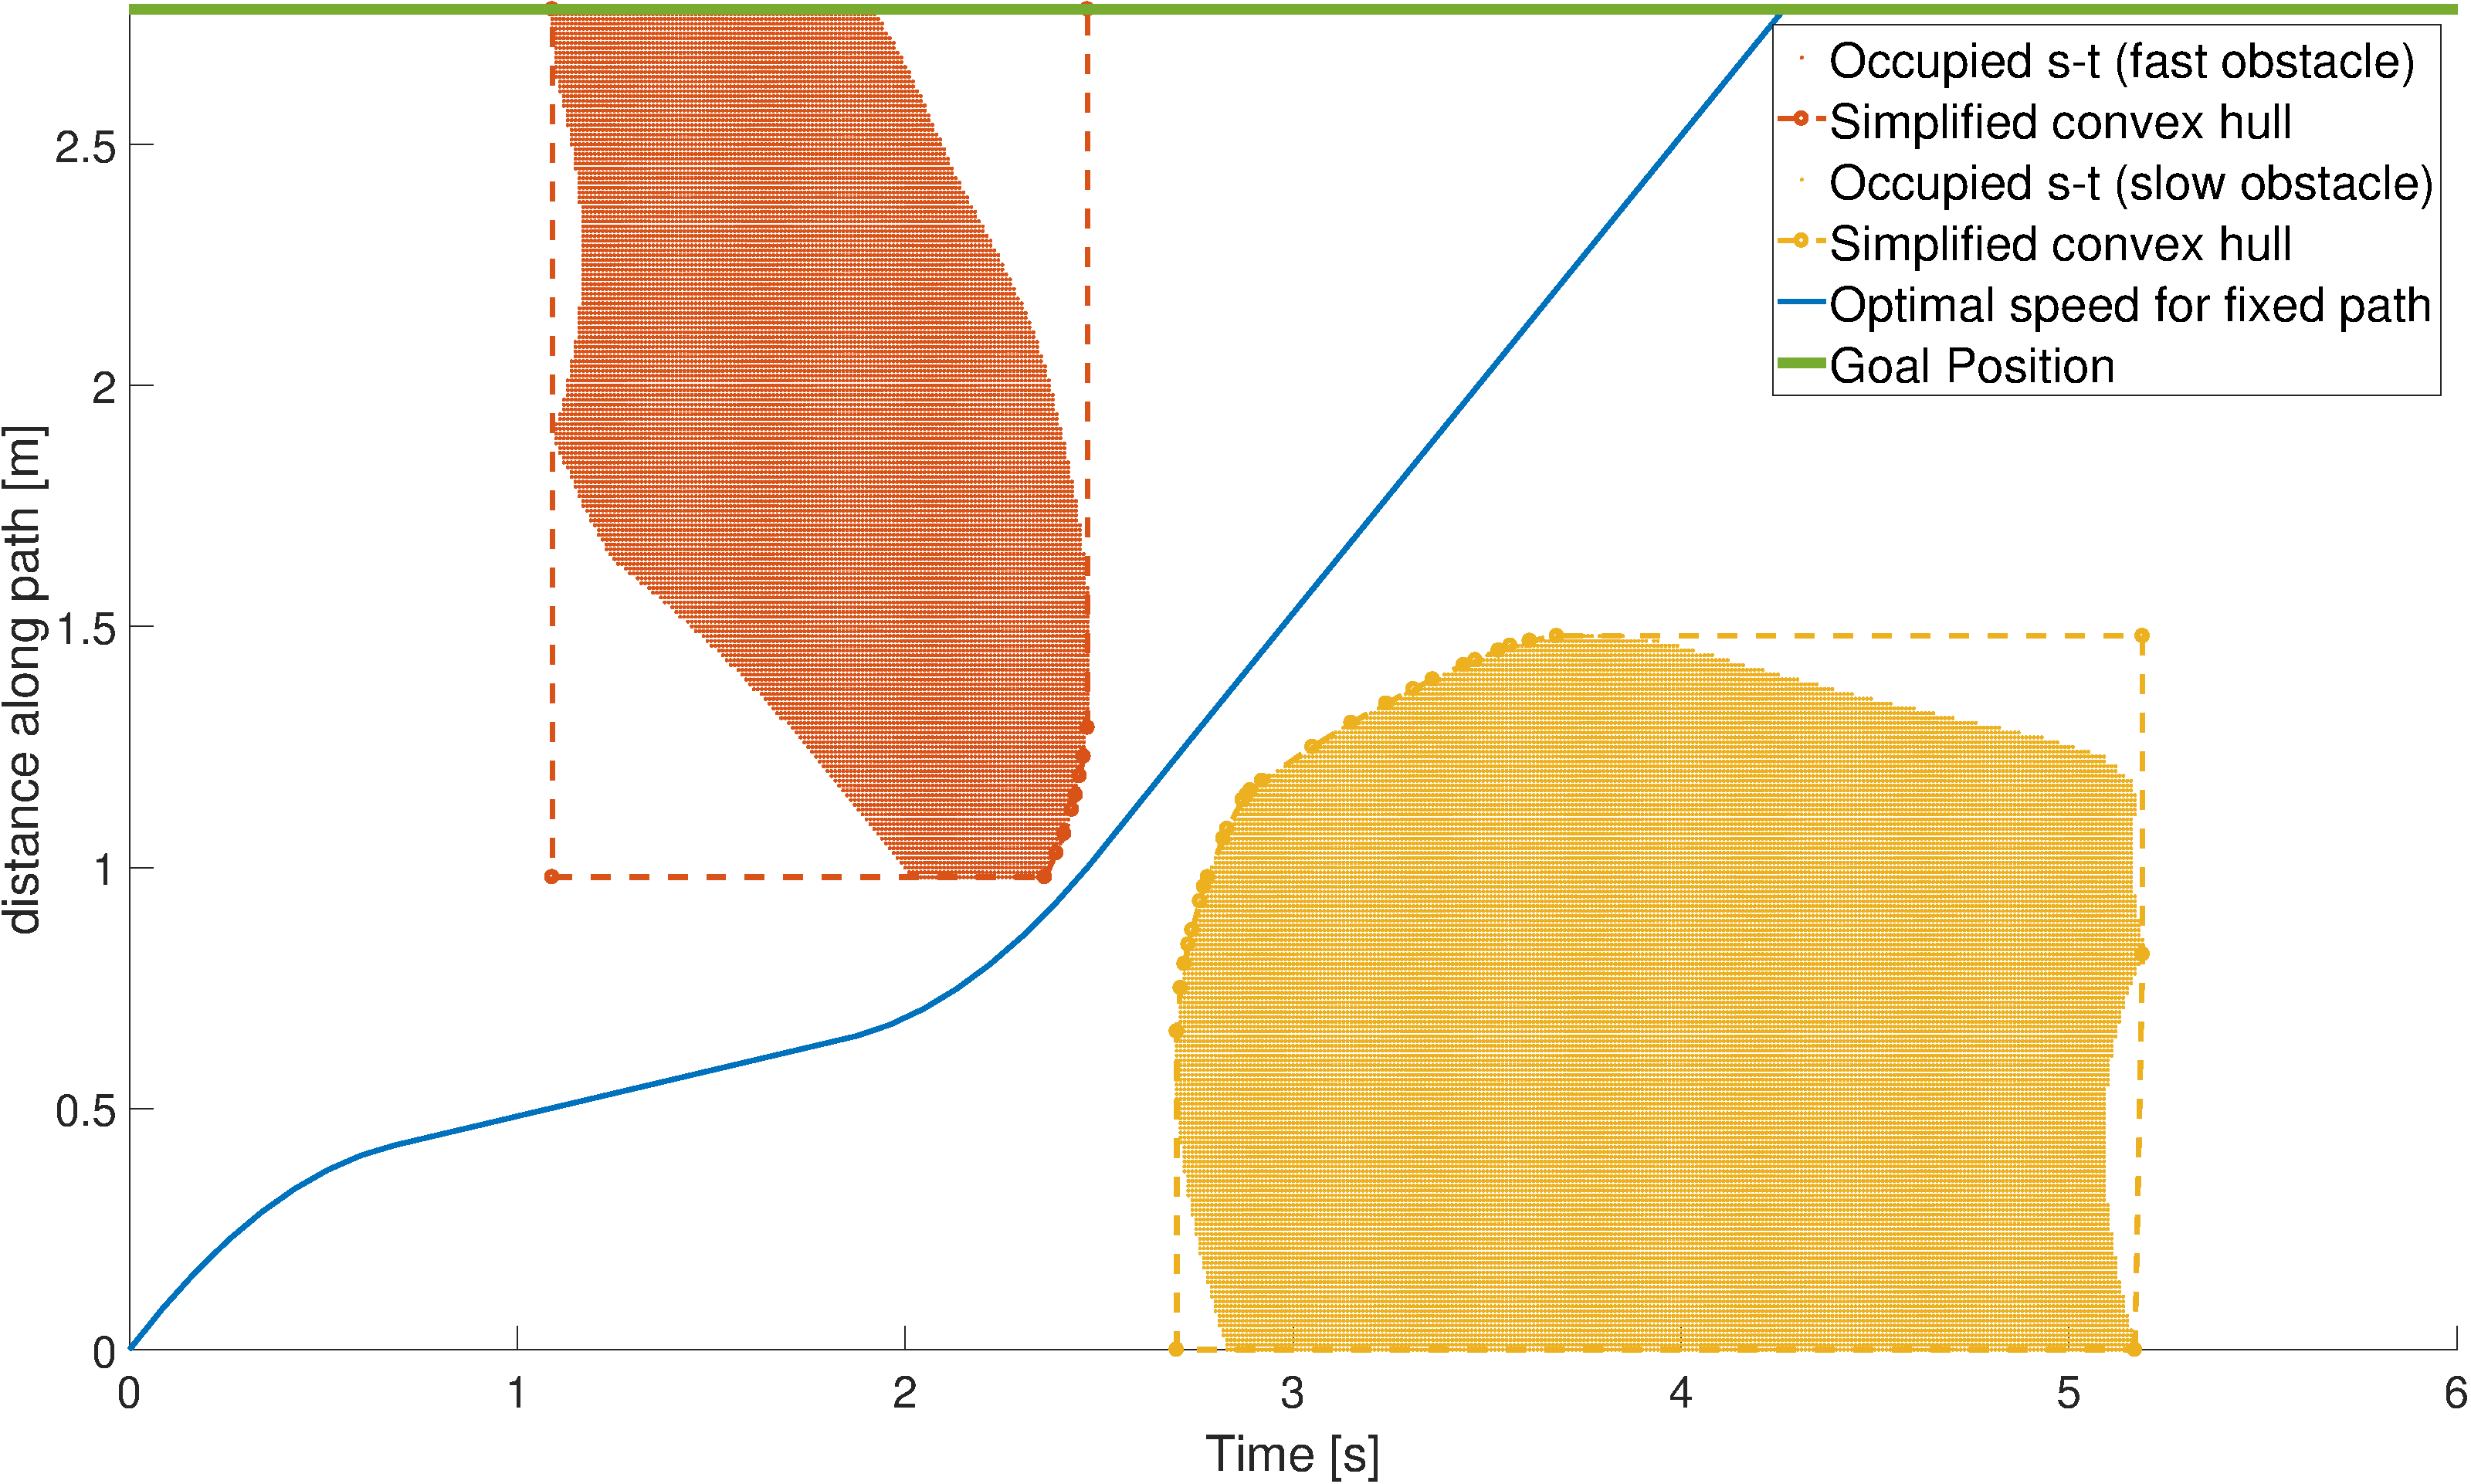
\includegraphics[width=\textwidth]{DVP_Solution.pdf}
\doublecaption{Dynamic motion planning among dynamic obstacles}{is achieved finding a path in the $s,t$-plane without intersecting the occupied cells. This results in an optimal speed profile for the sAMR, resulting in a collision-free motion.
\label{fig:DVP_Solution}}
\end{figure}


\newpage

\section{Socially Compliant Path Planning} \label{sec:HAPP}
The following section proposes solutions to different aspects reviewed in the literature study from \cref{sec:HARNrev} to obtain a path planner that will take into consideration several aspects of socially compliant navigation (\cref{sec:Comfort}).  An overview of the cooperation model developed by Trautman et al. \cite{TrautmanKrause2010,TrautmanEtAl2015} is given in \cref{sec:Cooperation} along with the most important mathematical models developed in their research. These additions have not been formally implemented in the source code presented in \cref{app:SourceCode}, but serve as guidelines in order to obtain a more socially compliant path planner.

\subsection{Enhancing comfort through social cost attribution} \label{sec:Comfort}
The impact on the comfort of humans with whom the driver and his wheelchair are interacting remains an important consideration even though the wheelchair is still guided by a person, as encoding those rules will make the planner inherently more socially acceptable. It is also possible that the driver has some disability making it more complicated for him to explicitly guide the wheelchair in a socially correct manner.

In order to obtain a path planner that inherently tries to follow social rules resulting in a more comfortable navigation as perceived by the surrounding people, a social cost should be computed for each path. After the intention of the driver has been calculated from the set of collision-free paths, weightings should be attributed to the path with the highest probability to be the user's intention and its associated social cost (a higher cost corresponds to a higher discomfort to the interacting person). The use of a cost function is preferred to the use of forbidden zones, since some situations require the wheelchair to enter someone’s intimate space in crowded spaces. 

A dynamic social cost map has been developed in \cite{ScandoloFraichard2011} starting from the guidelines of static personal space cost based on the study of proxemics \cite{Hall1966}. The authors have added other important factors, based on the back space of a person and his current motion direction. The use of back space puts an additional cost on moving right behind a person outside of his field of view. This additional cost during motion will adopt an elliptical form (rather than the circular form for static proxemics) and is proportional (and aligned) according to the velocity of the walking person.  This results in a dynamic personal space cost map displayed in \cref{fig:DynamicPersonalSpace}.

\begin{figure}[!htbp]
	\centering
    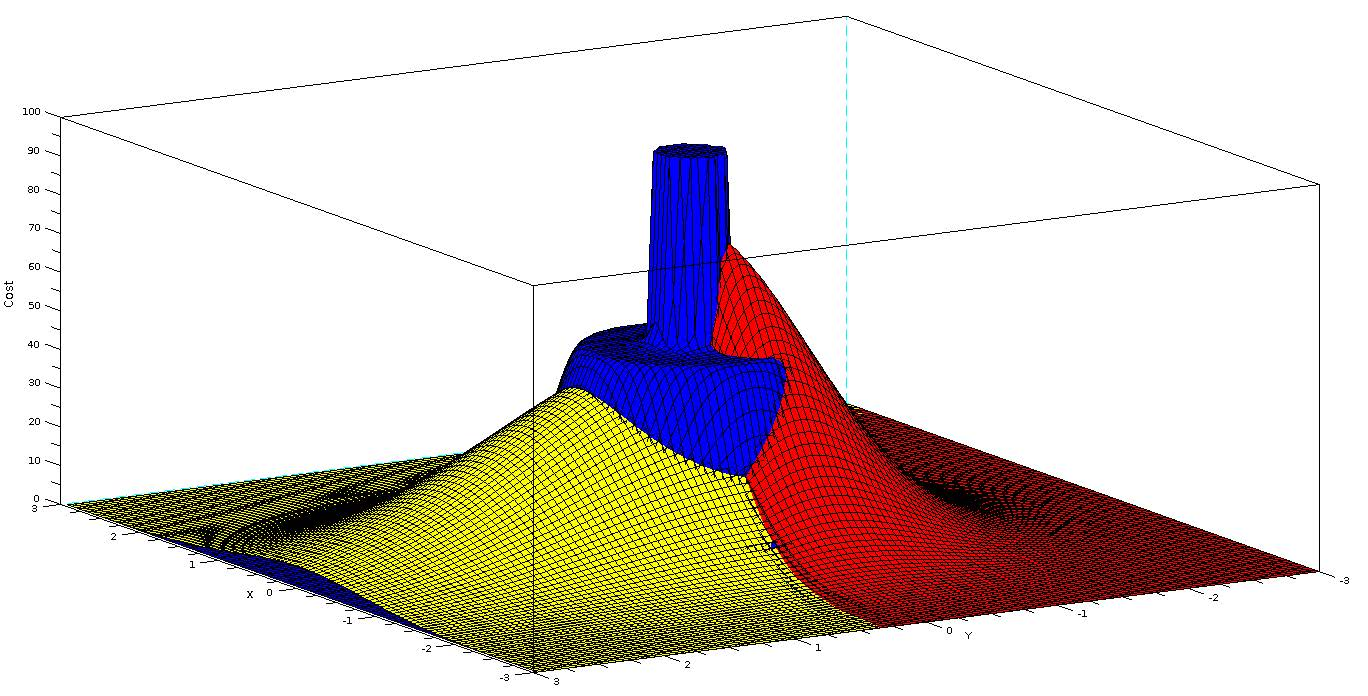
\includegraphics[width=0.5\textwidth]{DynamicPersonalSpace.jpg}
     \doublecaption{Dynamic personal space cost map.}{The blue area corresponds to the cost associated with the static proxemics. First, an infinite value is assigned to a distance resulting in a collision, followed by an exponential decrease depending on the different comfort zones (intimate, personal, social and public distance). The red area is the additional cost for being outside the field of view of the walking person. Finally, the yellow ellipse is the additional cost due to the motion of the person, reflecting the need to have a safe distance to stop (from \cite{ScandoloFraichard2011}).\label{fig:DynamicPersonalSpace}}
\end{figure}
 \vspace{-0.5em}
\subsection{Human-Robot Cooperation for Navigation in Crowed Spaces} \label{sec:Cooperation}
The research of Trautman et al. \cite{TrautmanKrause2010,TrautmanEtAl2015}, reviewed in \cref{sec:HRCrev}, has demonstrated that an independent motion planner will eventually fail even with perfect motion prediction of the agents surrounding the robot (recall \cref{fig:HuRoCo}). Eventually, when the density of a crowd of people exceeds a certain threshold, the planner will find no feasible paths and stop the robot or make it perform unnecessary evasive maneuvres. This is commonly called the FRP. Their solution to the FRP resides in the fact that people will adapt their own trajectories in order to make room for the wheelchair, thereby making it possible for everyone to reach their destination.

\begin{equation}
p_{\text{IGP}}({\bm f}^{(R)}, {\bm f^{(1:n)}}\vert {\bm z}_{1:t})=\frac{1}{Z}\psi({\bm f}^{(R)}, {\bm f^{(1:n)}})\prod\limits_{i=R}^{n}p({\bm f}^{(i)}\vert{\bm z}_{1:t}) \label{eq:IGPmodel}
\end{equation}

The developed prediction model, named Interacting Gaussian Process, is constructed by the interaction of the robot (${\bm f}^{(R)}$) and the other surrounding agents (${\bm f}^{(1:n)}$) with their corresponding observation (${\bm z}^{(1:n)}_{1:t}$), as displayed in \cref{eq:IGPmodel}. The probability over the whole trajectory from timesteps $1$ to $T$ (${\bm f}^{(i)} = f_{1}^{(i)}, \ldots, f_{T}^{({i})}$, $f^{(i)}_t = [x(t),y(t)]$) is modelled as a Gaussian Process. This Gaussian Process is defined by a mean function ($m^{(i)}$) and a kernel (covariance) function ($k^{(i)}$). The kernel function, which will model the shape of the agent's trajectories, is composed of a linear (nominal movement), Matern (mild curving) and noise (sensor noise) kernel. The different hyperparameters needed to define those terms are calculated based on training data (see \cite{TrautmanEtAl2015} for more information). The key function capturing the interaction between the agents is found in the interaction potential $\psi$ (see \cref{eq:InterPotFunc}), which requires only 2 tuning parameters: $h$ (controlling the ``safety margin'') and $\alpha$ (the strength of repulsion). $\vert f_{\tau}^{(i)}-f_{\tau}^{(j)}\vert$ is the Euclidean distance between agent $i$ and $j$ at time instance $\tau$. The interaction potential models the joint collision avoidance people adopt in crowded environments by lowering the provability a certain trajectory between two agents becomes from the moment they are too close to each other, since this would result in a possible collision between those two agents. $h$ and  $\alpha$ should be chosen in such a way that the minimal distance between two agents (observed from a training set) is enforced.

\begin{figure}[!tbp]
	\centering
    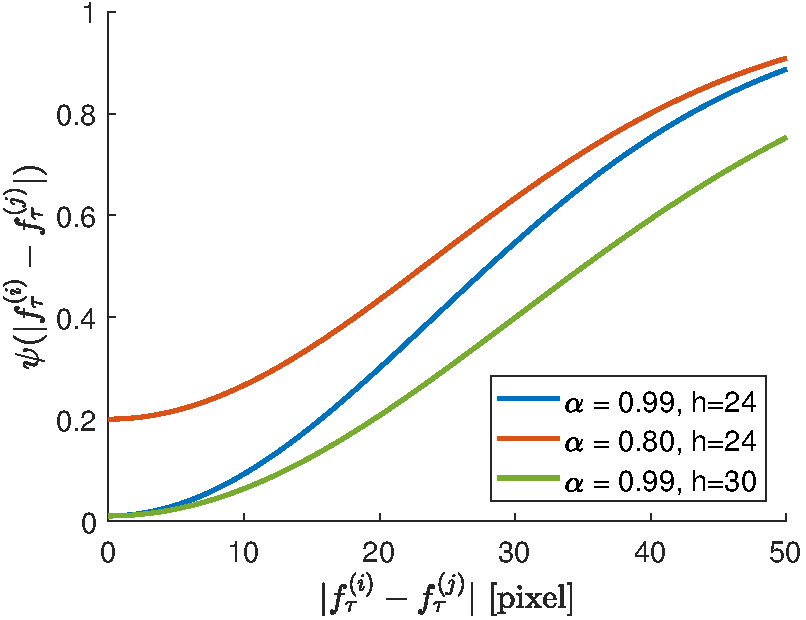
\includegraphics[width=0.5\textwidth]{InteractionPotentialFunction.pdf}
     \doublecaption{Influence of the two defining parameters for interaction potential between agent $i$ and $j$ at time instant $\tau$}{defined by \cref{eq:InterPotFunc}. ($\alpha$ and $h$) and is dependent on the (instantaneous) Euclidean distance between the two agents. This function lowers the probability that agent $i$ and $j$ are too close to each other at a given time instance $\tau$, reflecting the joint collision avoidance nature of humans. The distance is specified in pixels as an overhead camera was used during the experiments (adapted from \cite{TrautmanKrause2010}).\label{fig:InteractionPotentialFunction}}
\vspace{-1.5em}
\end{figure}

\begin{equation}
\psi({\bm f}^{(R)}, {\bm f^{(1:n)}})= \prod^{n}_{i=R}\prod^{n}_{j=i+1}\prod^{T}_{\tau=t}\left(1-\alpha\exp (-\frac{1}{2h^{2}}\vert f_{\tau}^{(i)}-f_{\tau}^{(j)}\vert)\right) \label{eq:InterPotFunc}
\end{equation}

From the derived model, one can design a LPPA that anticipates cooperation from the surrounding agents. However, ultimately, the observation ${\bm z}^{(1:n)}_{1:t}$ will still take priority, in case of non-cooperation. The path planning action is obtained by finding the maximum a posteriori from \cref{eq:IGPmodel} and by taking $f_{t+1}^{(R)\,\ast}$ as next waypoint for the navigation module, until the robot has arrived at its destination, shown in \cref{eq:NavMAP}.

\begin{equation}
({\bm f}^{(R)}, {\bm f^{(1:n)}})^{\ast}=\arg\max_{{\bm f}^{(R)},{\bm f^{(1:n)}}} P_{\text{IGP}} ({\bm f}^{(R)}, {\bm f^{(1:n)}}\vert {\bm z}_{1:t}) \label{eq:NavMAP}
\end{equation}

\section{Conclusion} \label{sec:DesignConclusion}
The developed clothoidal LPT uses a less restrictive curve geometry compared to the circular LPT used in \cite{DemeesterEtAl2012}, therefore providing a larger set of feasible paths. In situations where the sAMR has to travel through narrow openings, the clothoidal LPT will have a higher probability to find feasible paths, therefore providing better navigation assistance to the user of the wheelchair. The calculated paths connect the origin with discrete end poses in the surroundings of the robot, whilst taking into account the robot's constraints. 

Two alternatives have been compared to build the curve geometry, the Bézier curve and the clothoid. The latter has been selected for mainly two reasons: (i) it has a less restrictive formulation compared to the circle, since the curvature can vary linearly w.r.t. the path length; (ii) when driving at constant speed, the rotation speed of the wheels will only have to change linearly, making the clothoid easier to follow compared to the Bézier curve. To provide an even wider set of feasible paths, some paths consist of two clothoids. 

By using a predefined set of paths, the space the wheelchair will take along each path is known in advance and can be stored in a precomputed lookup table. The structure of the lookup table is optimized by containing for each occupied grid cell of the LPT the different paths occupying that certain grid cell and all the respective path lengths (when occupying that particular grid). In the online phase, the LPPA only has to compare the occupied cells from the grid-map containing all the obstacles of the environment with the lookup table. Each occupied cell will influence the total length of each path if the path length is shortened. It is important to note that the shape of both the robot and the obstacle can be arbitrary (convex or concave), but have to be converted in a grid-map.

A conceptual solution has been put forward for the calculation of the velocity profile when taking a path. The solution is based on the construction of an efficient search space in the distance-time collision space, relying on the fixed nature of the LPT and a given motion model of an obstacle to find a collision-free motion, compliant with the kinematic and dynamic constraints of the wheelchair. This efficient search-space has another interesting feature, notably the relative similarity of the collision-space occupied cells for similar paths, enabling grid search methods with a re-planning ability (e.g. D* or Incremental Phi*) to find quickly a solution for similar paths. 

Socially compliant path planning can take the shape of social costs resulting from the interaction of the user and his wheelchair with other individuals or crowds which can be attributed to selected paths. Whilst this additional social costing has not been formally implemented in the local path planning design as developed under \Cref{app:SourceCode}, such methodology remains compatible with the design of the clothoidal LPT. The human-robot cooperation model demonstrates promising results since it tackles one of the most important aspects in human navigation, the joint collision avoidance people engage in when walking in dense crowds. Without considering human behavior, the autonomous assisted navigation will not function properly in crowded environments.

By expanding the set of feasible paths of the LPT it is crucial to quantify the extra time needed when performing the online collision checking algorithm.  An in-depth evaluation of the clothoidal LPT will be discussed in \cref{cha:Eval}, by comparing it to the circular LPT.